\documentclass[a4paper,11pt]{report}
\usepackage{psfrag}
\usepackage[showexo=true,showcorr=false,showdegree=true]{../packages/coursclassed}
%Commenter ou enlever le commentaire sur la ligne suivante pour montrer le niveau
\toggletrue{montrerNiveaux}
%permet de gérer l'espacement entre les items des env enumerate et enumitem
\usepackage{enumitem}
\setlist[enumerate]{align=left,leftmargin=1cm,itemsep=10pt,parsep=0pt,topsep=0pt,rightmargin=0.5cm}
\setlist[itemize]{align=left,labelsep=1em,leftmargin=*,itemsep=0pt,parsep=0pt,topsep=0pt,rightmargin=0cm}
%permet de gerer l'espacement entre les colonnes de multicols
\setlength\columnsep{35pt}

\begin{document}

%%%%%%%%%%%%%%%%% À MODIFIER POUR CHAQUE SERIE %%%%%%%%%%%%%%%%%%%%%%%%%%%%%
\newcommand{\chapterName}{Fonctions et algèbre}
\newcommand{\serieName}{Introduction aux fonctions}

%%%%%%%%%%%%%%%%%% PREMIERE PAGE NE PAS MODIFER %%%%%%%%%%%%%%%%%%%%%%%%
% le chapitre en cours, ne pas changer au cours d'une série
\chapter*{\chapterName}
\thispagestyle{empty}
%
%%%%%% LISTE AIDE MEMOIRE %%%%%%
\begin{amL}{\serieName}{
\item Fonctions - Généralités (page 46)
\item Représentation graphique (page 46)
\item Définir une fonction (page 47)
\item Fonction affine (page 48)
}\end{amL}

%%%%%%%%%%%%%%% DEBUT DE LA SERIE NE PAS MODIFIER %%%%%%%%%%%%%%%%%%%%%%%%%%%%%
\section*{\serieName}
\setcounter{page}{1}

%%%%%%%%%%% LES EXERCICES %%%%%%%%%%%%%%%%%%%%%%%%%%%%%%%%%%%%
\resolu{Boites noires}{Complète les boîtes noires ci-dessous :
\vspace*{.25cm}
%
%\begin{minipage}{0.3 \linewidth}
%\psfrag{a}{$0 $}
%\psfrag{A}{$ 0$}
%\psfrag{b}{$ 2$}
%\psfrag{B}{$ 4$}
%\psfrag{c}{$ 5$}
%\psfrag{C}{$ 10$}
%\psfrag{d}{$ -3$}
%\psfrag{D}{$-6 $}
%\psfrag{e}{$a$}
%\psfrag{E}{$ 2a$}
%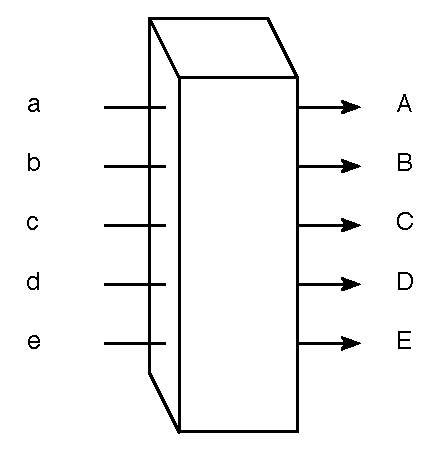
\includegraphics[scale=.6]{media/FA-30/boitenoire5.eps}
%\end{minipage} \hfill
%\begin{minipage}{0.3\linewidth}
%\psfrag{a}{$ 0$}
%\psfrag{A}{$5 $}
%\psfrag{b}{$ 1$}
%\psfrag{B}{$6 $}
%\psfrag{c}{$-2 $}
%\psfrag{C}{$3 $}
%\psfrag{d}{$ 9$}
%\psfrag{D}{$14 $}
%\psfrag{e}{$b$}
%\psfrag{E}{$b+5 $}
%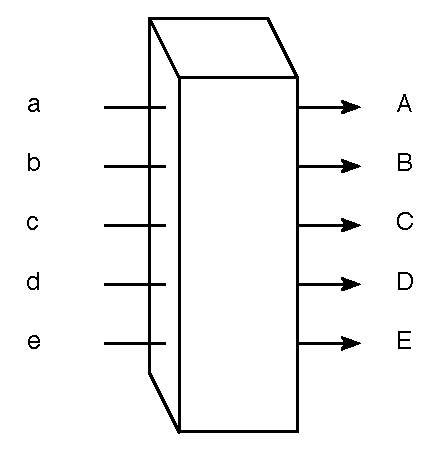
\includegraphics[scale=.6]{media/FA-30/boitenoire5.eps}
%\end{minipage}
%\hfill
%\begin{minipage}{0.3\linewidth}
%\psfrag{a}{$0 $}
%\psfrag{A}{$ -2$}
%\psfrag{b}{$4 $}
%\psfrag{B}{$ 10$}
%\psfrag{c}{$-2 $}
%\psfrag{C}{$ -8$}
%\psfrag{d}{$5 $}
%\psfrag{D}{$13 $}
%\psfrag{e}{$c$}
%\psfrag{E}{$3c-2$}
%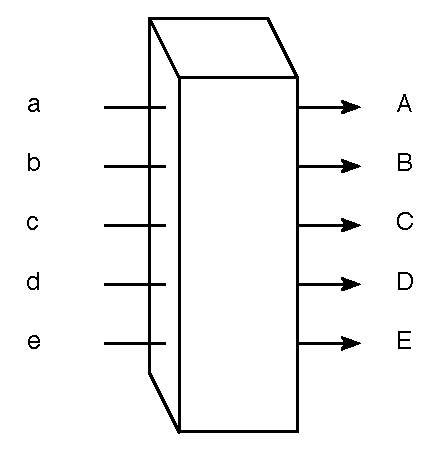
\includegraphics[scale=.6]{media/FA-30/boitenoire5.eps}
%\end{minipage}
%
%\vspace*{.75cm}
%
%\begin{minipage}{0.3 \linewidth}
%\psfrag{a}{$0 $}
%\psfrag{A}{$ 0$}
%\psfrag{b}{$ 3$}
%\psfrag{B}{$ -3$}
%\psfrag{c}{$ -5$}
%\psfrag{C}{$ 5$}
%\psfrag{d}{$ -3$}
%\psfrag{D}{$3 $}
%\psfrag{e}{$x$}
%\psfrag{E}{$ -x$}
%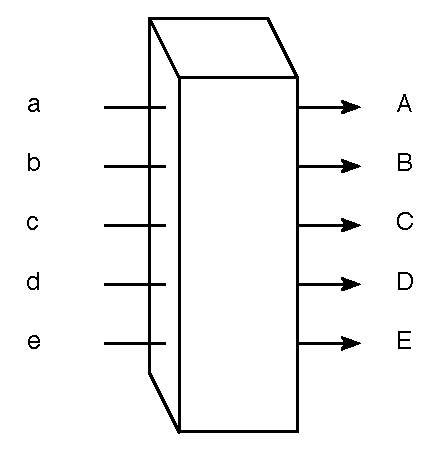
\includegraphics[scale=.6]{media/FA-30/boitenoire5.eps}
%\end{minipage} \hfill
%\begin{minipage}{0.3\linewidth}
%\psfrag{a}{$ 0$}
%\psfrag{A}{$0 $}
%\psfrag{b}{$ 0,\!5$}
%\psfrag{B}{$0,\!25 $}
%\psfrag{c}{$-2 $}
%\psfrag{C}{$4 $}
%\psfrag{d}{$ 7$}
%\psfrag{D}{$49 $}
%\psfrag{e}{$y$}
%\psfrag{E}{$y^2 $}
%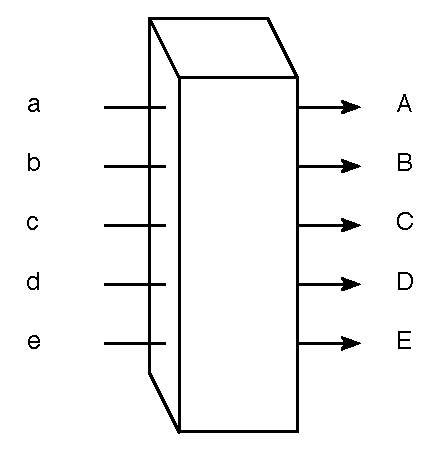
\includegraphics[scale=.6]{media/FA-30/boitenoire5.eps}
%\end{minipage}
%\hfill
%\begin{minipage}{0.3\linewidth}
%\psfrag{a}{$1 $}
%\psfrag{A}{$ -5$}
%\psfrag{b}{$20 $}
%\psfrag{B}{$ -5$}
%\psfrag{c}{$-8 $}
%\psfrag{C}{$ -5$}
%\psfrag{d}{$5 $}
%\psfrag{D}{$-5 $}
%\psfrag{e}{$z$}
%\psfrag{E}{$-5$}
%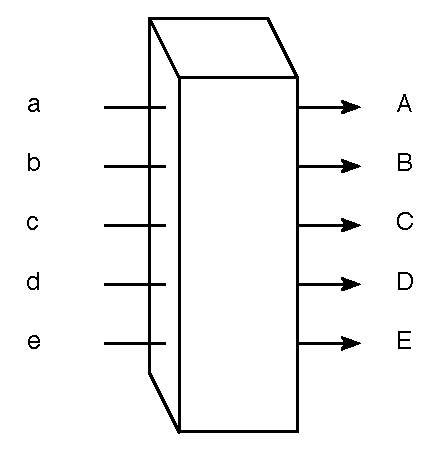
\includegraphics[scale=.6]{media/FA-30/boitenoire5.eps}
%\end{minipage}
%%%%%%%%% Fin de la version en eps avec PSFRAG%%%%%%%%%%%%%%%%%%%%%%%%%%%%%%%%%%%%%
\begin{center}
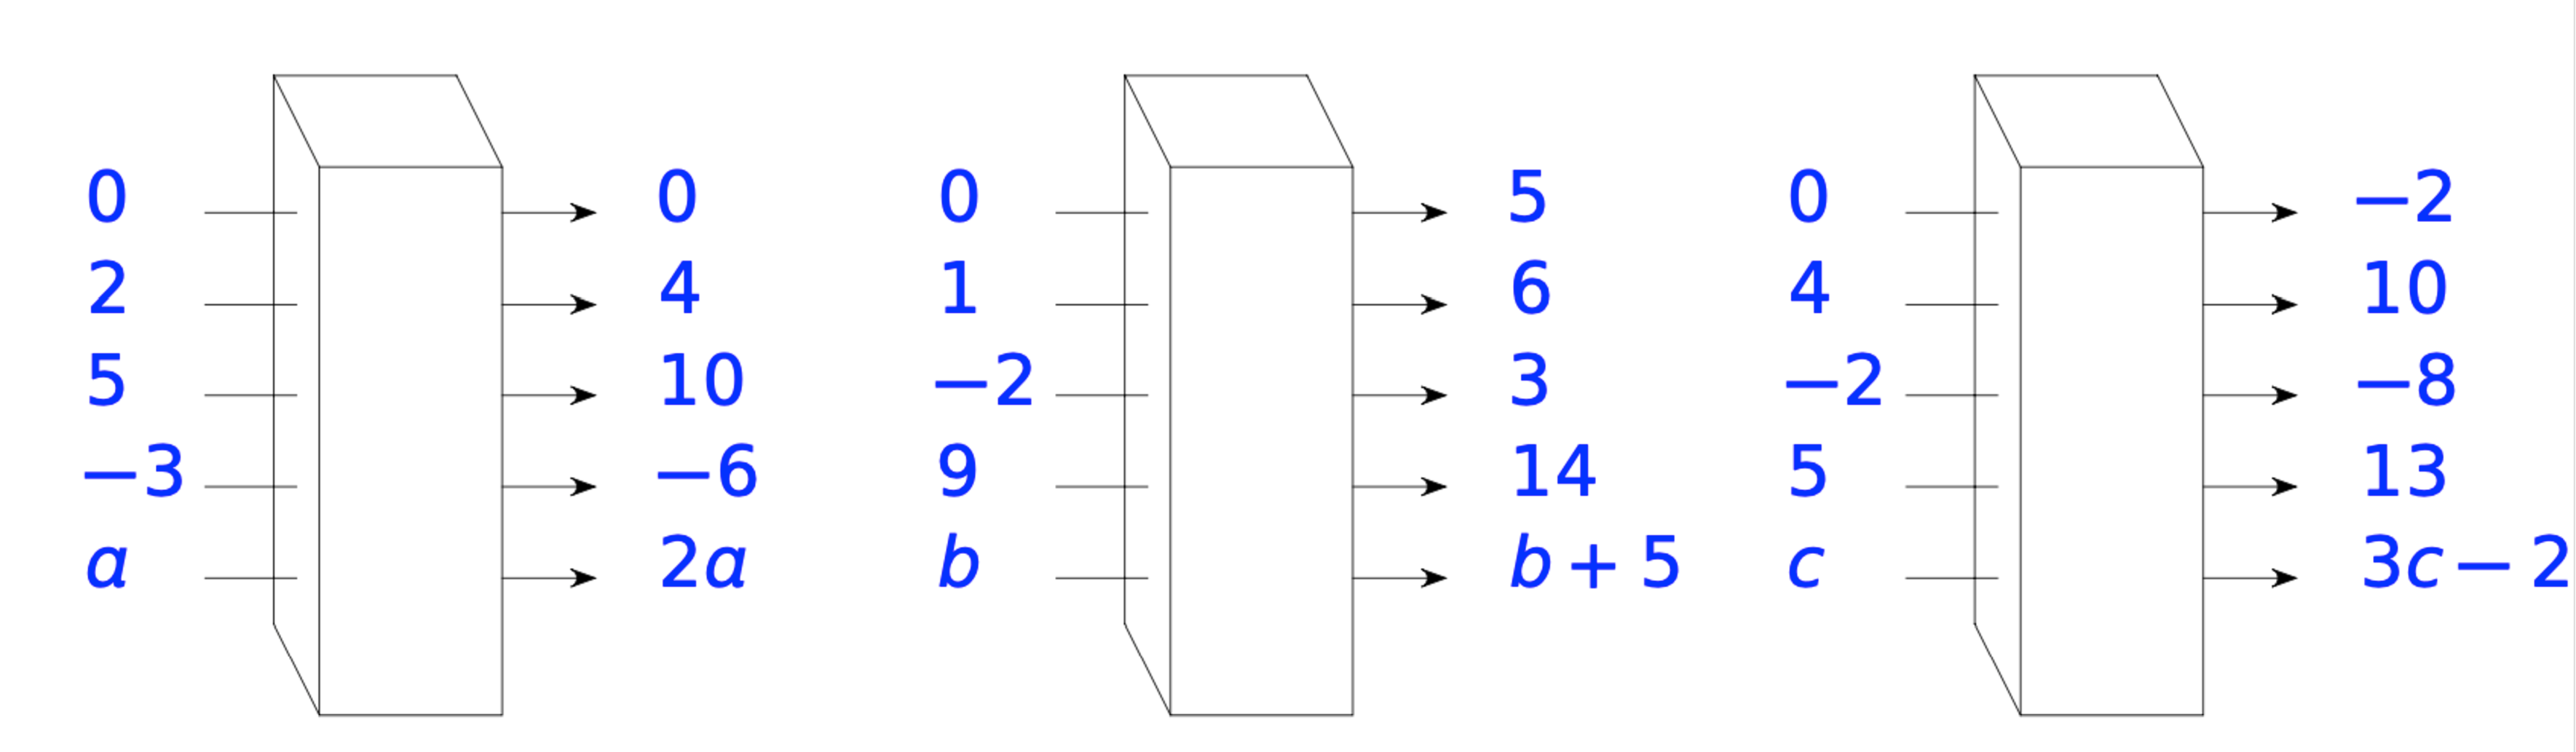
\includegraphics[width=1\textwidth]{media/FA-30/bn1.pdf}
\end{center}
\bigskip
\begin{center}
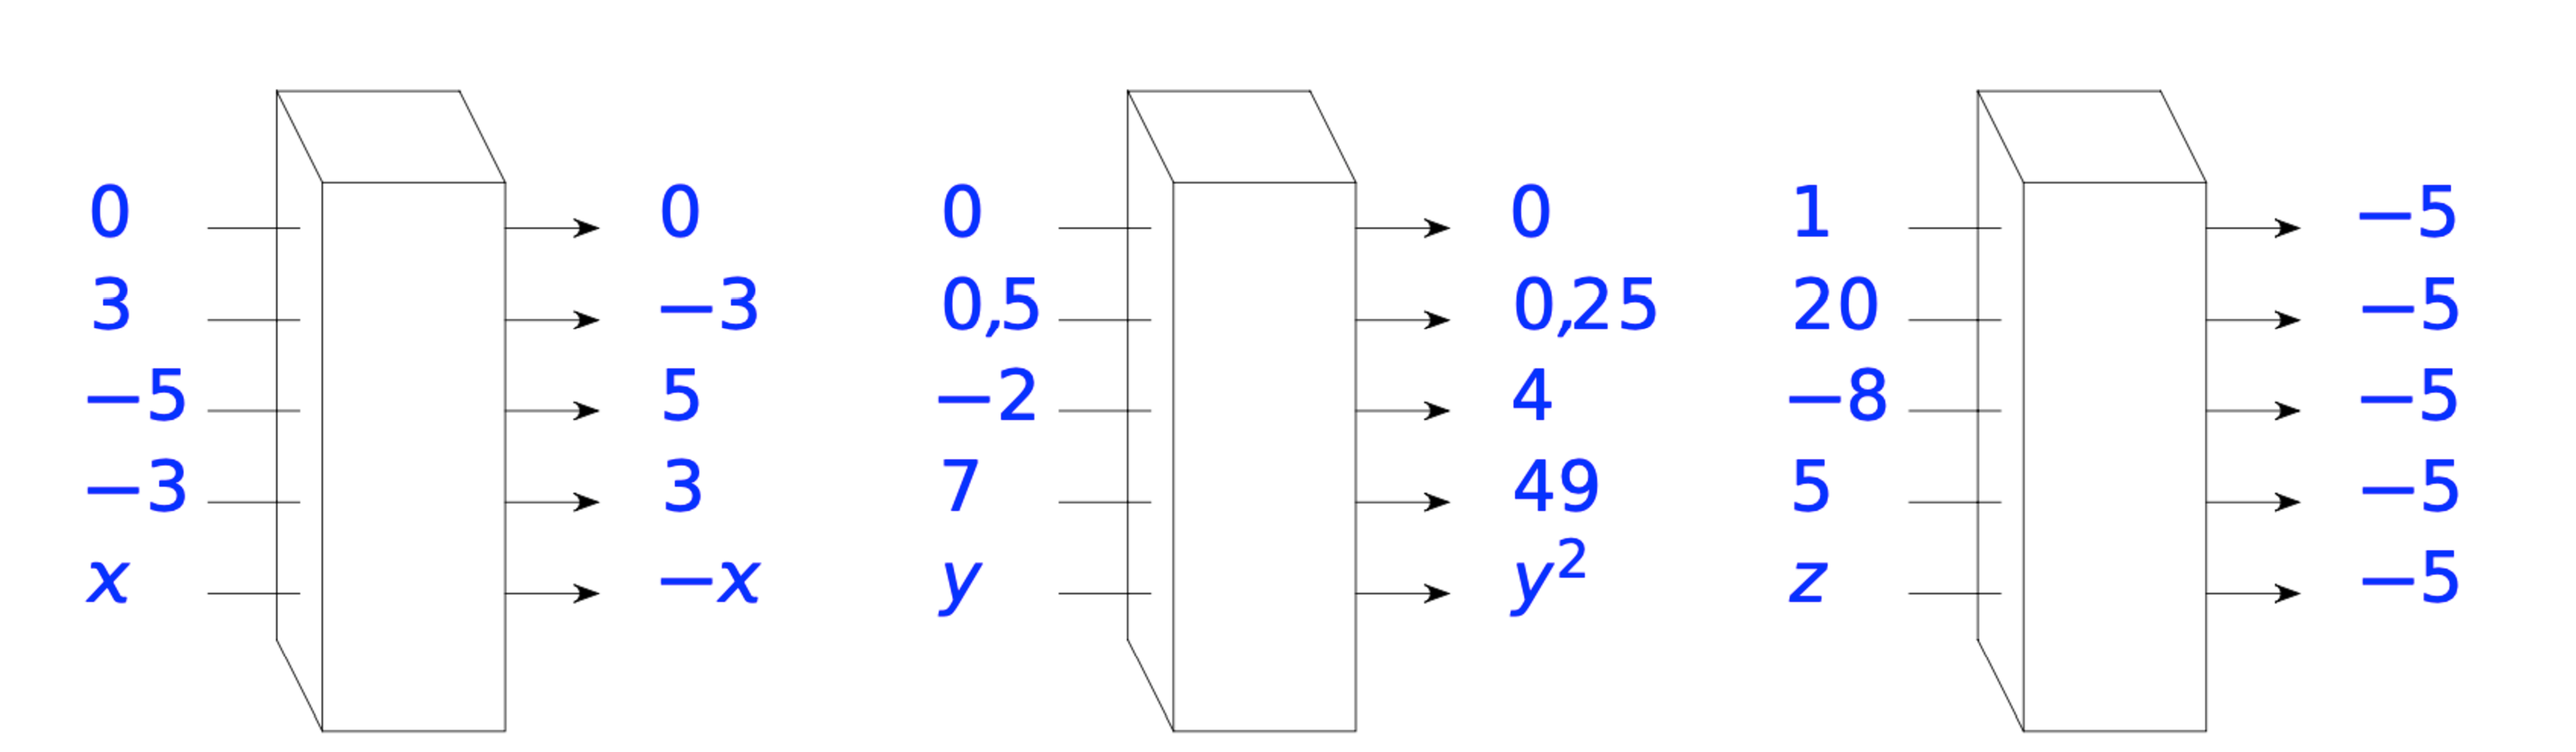
\includegraphics[width=1\textwidth]{media/FA-30/bn2.pdf}
\end{center}

\smallskip

Il faut s'imaginer une fonction comme une machine ou une boîte noire qui  effectue une chaîne d'opérations définie lorsqu'on lui rentre un nombre et nous retourne le résultat correspondant à ce nombre de départ.
}
{2}

\newpage

\exop{Complète les boîtes noires ci-dessous :
\vspace*{.75cm}
%%%% Boites noires en EPS avec PSFRAG %%%%%%%%%%
%\begin{minipage}{0.3 \linewidth}
%\psfrag{a}{$0 $}
%\psfrag{A}{\ligne{1}}
%\psfrag{b}{\ligne{1}}
%\psfrag{B}{$ 3$}
%\psfrag{c}{$ 4$}
%\psfrag{C}{\ligne{1}}
%\psfrag{d}{\ligne{1}}
%\psfrag{D}{$-6 $}
%\psfrag{e}{$a$}
%\psfrag{E}{$ 3a$}
%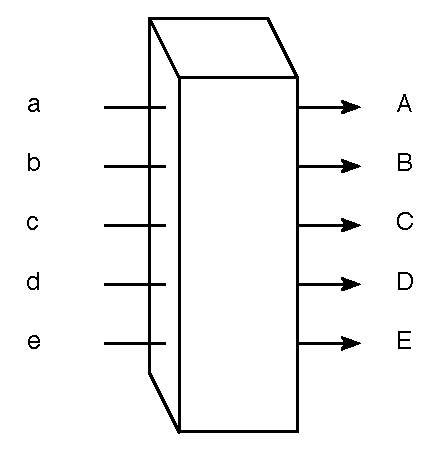
\includegraphics[scale=.6]{media/FA-30/boitenoire5.eps}
%\end{minipage} \hfill
%\begin{minipage}{0.3\linewidth}
%\psfrag{a}{\ligne{1}}
%\psfrag{A}{$-4 $}
%\psfrag{b}{$ 1$}
%\psfrag{B}{\ligne{1}}
%\psfrag{c}{$-2 $}
%\psfrag{C}{\ligne{1}}
%\psfrag{d}{\ligne{1}}
%\psfrag{D}{$-14 $}
%\psfrag{e}{$b$}
%\psfrag{E}{$b-4 $}
%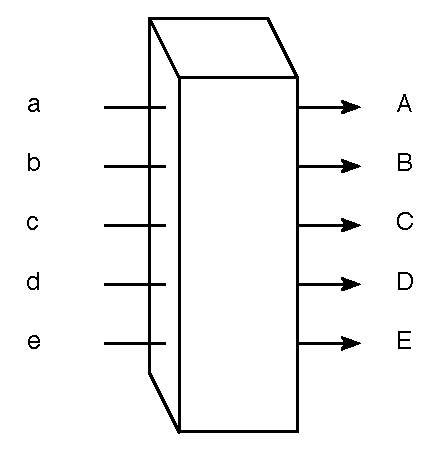
\includegraphics[scale=.6]{media/FA-30/boitenoire5.eps}
%\end{minipage}
%\hfill
%\begin{minipage}{0.3\linewidth}
%\psfrag{a}{$0 $}
%\psfrag{A}{\ligne{1}}
%\psfrag{b}{$4 $}
%\psfrag{B}{\ligne{1}}
%\psfrag{c}{\ligne{1}}
%\psfrag{C}{$ -7$}
%\psfrag{d}{$5 $}
%\psfrag{D}{\ligne{1}}
%\psfrag{e}{$c$}
%\psfrag{E}{$2c+1$}
%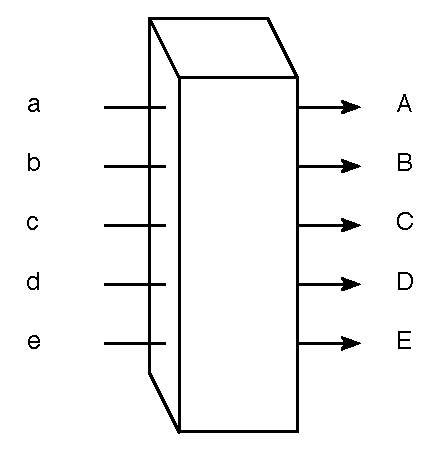
\includegraphics[scale=.6]{media/FA-30/boitenoire5.eps}
%\end{minipage}
%
%\vspace*{.75cm}
%
%\begin{minipage}{0.3 \linewidth}
%\psfrag{a}{$0 $}
%\psfrag{A}{\ligne{1}}
%\psfrag{b}{\ligne{1}}
%\psfrag{B}{$ -6$}
%\psfrag{c}{$ -8$}
%\psfrag{C}{\ligne{1}}
%\psfrag{d}{\ligne{1}}
%\psfrag{D}{$10 $}
%\psfrag{e}{$x$}
%\psfrag{E}{$ -2x$}
%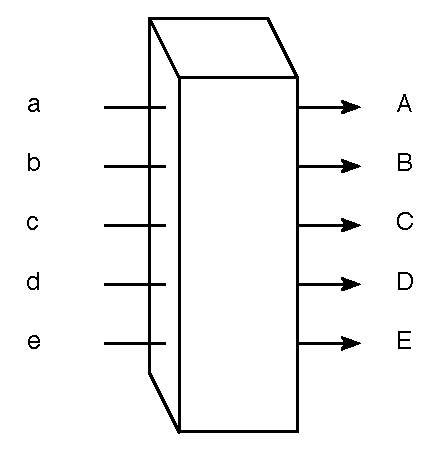
\includegraphics[scale=.6]{media/FA-30/boitenoire5.eps}
%\end{minipage} \hfill
%\begin{minipage}{0.3\linewidth}
%\psfrag{a}{$ 0$}
%\psfrag{A}{\ligne{1}}
%\psfrag{b}{\ligne{1}}
%\psfrag{B}{$8$}
%\psfrag{c}{\ligne{1}}
%\psfrag{C}{27}
%\psfrag{d}{$-4$}
%\psfrag{D}{$-64 $}
%\psfrag{e}{$y$}
%\psfrag{E}{$y^3 $}
%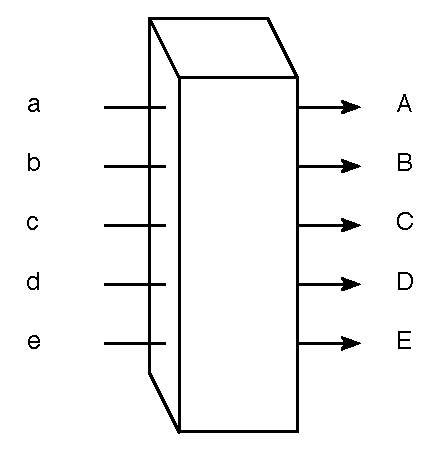
\includegraphics[scale=.6]{media/FA-30/boitenoire5.eps}
%\end{minipage}
%\hfill
%\begin{minipage}{0.3\linewidth}
%\psfrag{a}{\ligne{1}}
%\psfrag{A}{$ -2$}
%\psfrag{b}{$20 $}
%\psfrag{B}{\ligne{1}}
%\psfrag{c}{$-8 $}
%\psfrag{C}{\ligne{1}}
%\psfrag{d}{$5 $}
%\psfrag{D}{\ligne{1}}
%\psfrag{e}{$z$}
%\psfrag{E}{$-2$}
%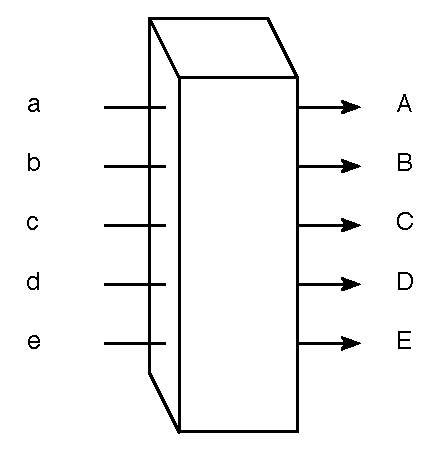
\includegraphics[scale=.6]{media/FA-30/boitenoire5.eps}
%\end{minipage}
%%%% FIN DES BOITES NOIRES EN EPS AVEC PSFRAG %%%%%%%%%%%%%%%%%%%%%%%%%%%%%%%%%%%
\begin{center}
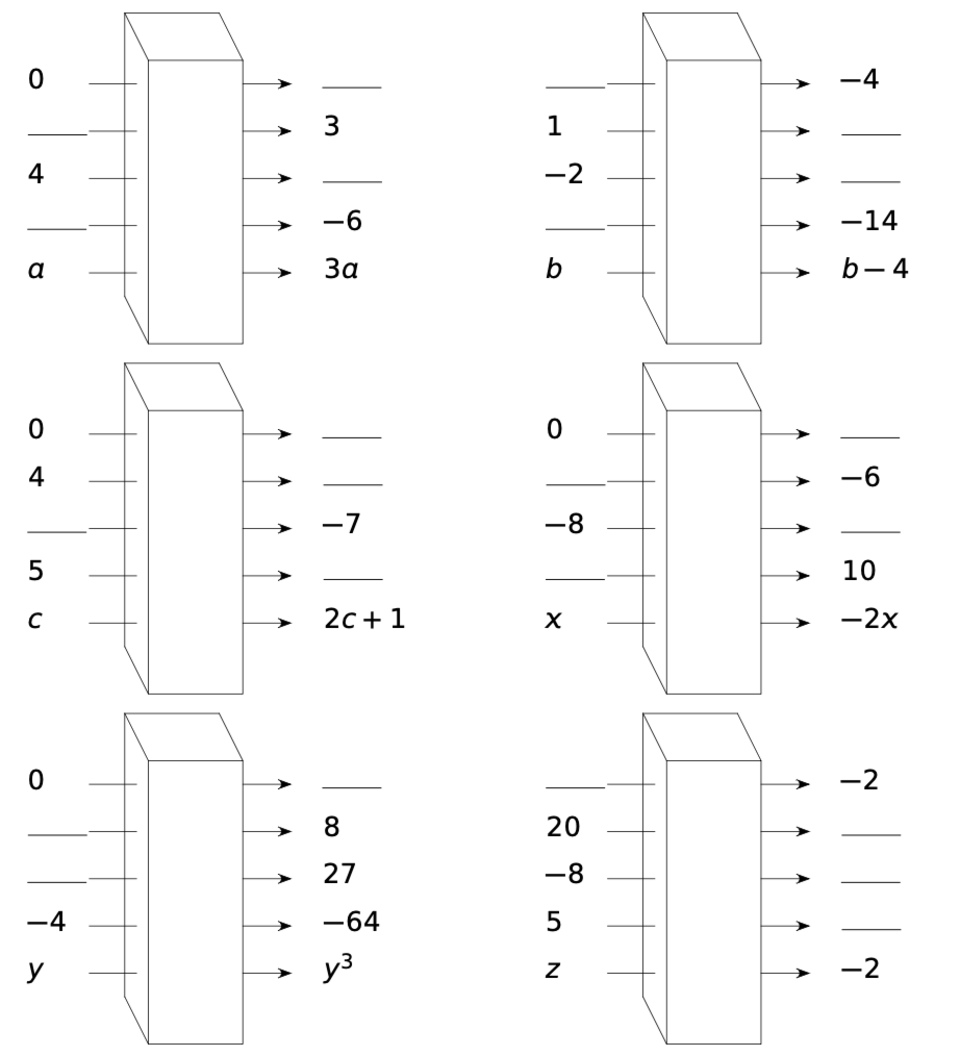
\includegraphics[width=1\textwidth]{media/FA-30/bn10.pdf}
\end{center}
%\bigskip
%\begin{center}
%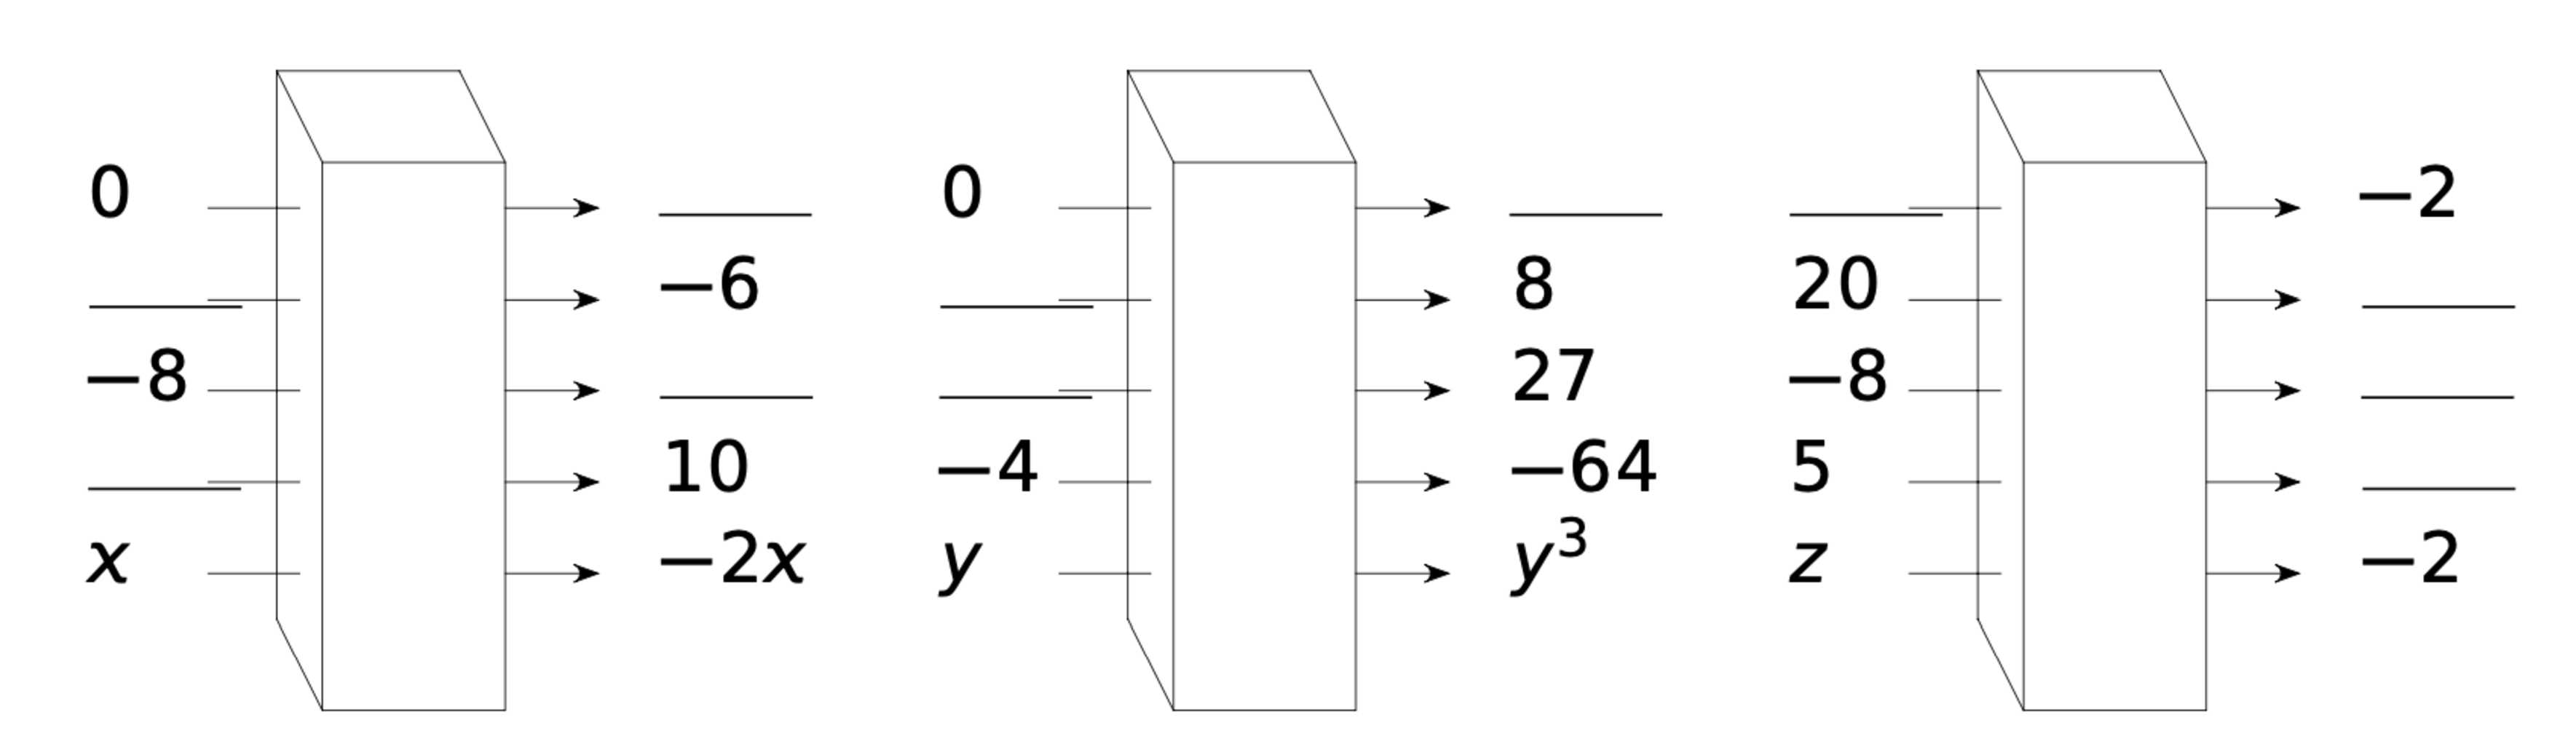
\includegraphics[width=1\textwidth]{media/FA-30/bn4.pdf}
%\end{center}
}
{2}

\newpage


\exop{Complète les boîtes noirs ci-dessous :
\vspace*{.75cm}
%%%%% BOITES NOIRES EN EPS AVEC PSFRAG %%%%%%
%\begin{minipage}{0.3 \linewidth}
%\psfrag{a}{$0 $}
%\psfrag{A}{\ligne{1}}
%\psfrag{b}{\ligne{1}}
%\psfrag{B}{$ 15$}
%\psfrag{c}{$ 4$}
%\psfrag{C}{\ligne{1}}
%\psfrag{d}{\ligne{1}}
%\psfrag{D}{$-20 $}
%\psfrag{e}{$a$}
%\psfrag{E}{$ 5a$}
%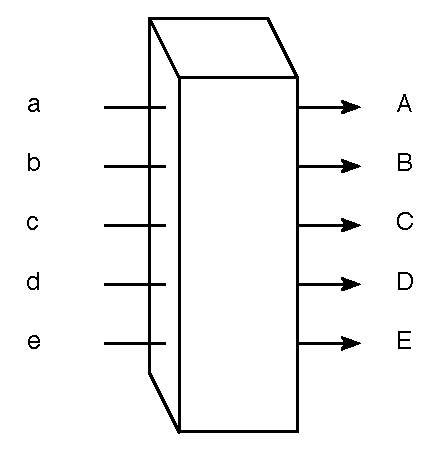
\includegraphics[scale=.6]{media/FA-30/boitenoire5.eps}
%\end{minipage} \hfill
%\begin{minipage}{0.3\linewidth}
%\psfrag{a}{\ligne{1}}
%\psfrag{A}{$-2 $}
%\psfrag{b}{$ 1$}
%\psfrag{B}{\ligne{1}}
%\psfrag{c}{$-5 $}
%\psfrag{C}{\ligne{1}}
%\psfrag{d}{\ligne{1}}
%\psfrag{D}{$14 $}
%\psfrag{e}{$b$}
%\psfrag{E}{$b+7 $}
%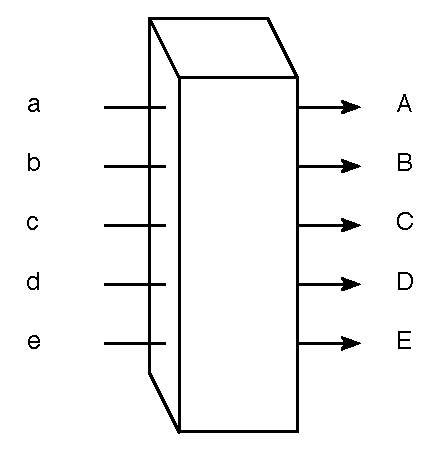
\includegraphics[scale=.6]{media/FA-30/boitenoire5.eps}
%\end{minipage}
%\hfill
%\begin{minipage}{0.3\linewidth}
%\psfrag{a}{$0 $}
%\psfrag{A}{\ligne{1}}
%\psfrag{b}{$2 $}
%\psfrag{B}{\ligne{1}}
%\psfrag{c}{\ligne{1}}
%\psfrag{C}{$ -17$}
%\psfrag{d}{$6 $}
%\psfrag{D}{\ligne{1}}
%\psfrag{e}{$c$}
%\psfrag{E}{$4c+3$}
%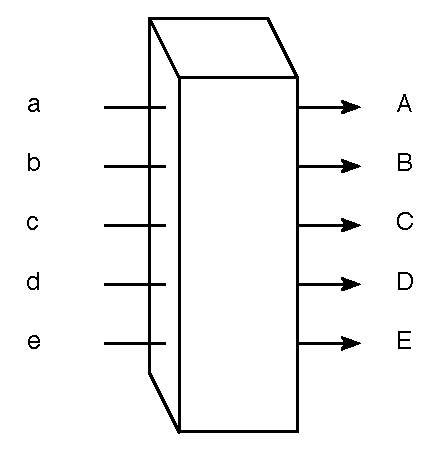
\includegraphics[scale=.6]{media/FA-30/boitenoire5.eps}
%\end{minipage}
%
%\vspace*{.75cm}
%
%\begin{minipage}{0.3 \linewidth}
%\psfrag{a}{$0 $}
%\psfrag{A}{\ligne{1}}
%\psfrag{b}{\ligne{1}}
%\psfrag{B}{$ -6$}
%\psfrag{c}{$ -8$}
%\psfrag{C}{\ligne{1}}
%\psfrag{d}{\ligne{1}}
%\psfrag{D}{$30 $}
%\psfrag{e}{$x$}
%\psfrag{E}{$ -3x$}
%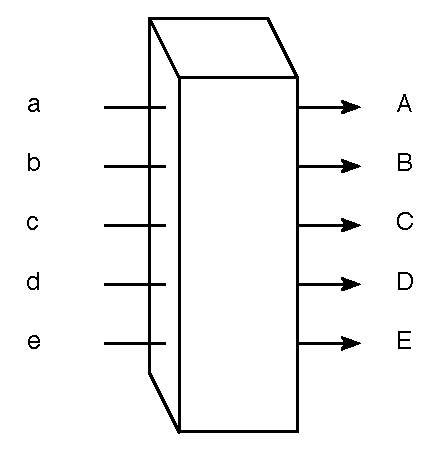
\includegraphics[scale=.6]{media/FA-30/boitenoire5.eps}
%\end{minipage} \hfill
%\begin{minipage}{0.3\linewidth}
%\psfrag{a}{$ 0$}
%\psfrag{A}{\ligne{1}}
%\psfrag{b}{\ligne{1}}
%\psfrag{B}{$8$}
%\psfrag{c}{\ligne{1}}
%\psfrag{C}{50}
%\psfrag{d}{$-$}
%\psfrag{D}{$ $}
%\psfrag{e}{$y$}
%\psfrag{E}{$2y^2 $}
%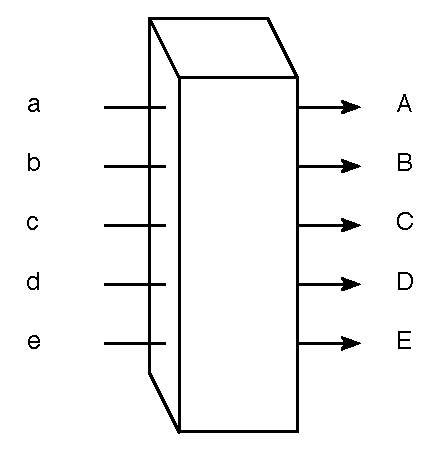
\includegraphics[scale=.6]{media/FA-30/boitenoire5.eps}
%\end{minipage}
%\hfill
%\begin{minipage}{0.3\linewidth}
%\psfrag{a}{\ligne{1}}
%\psfrag{A}{$ -7$}
%\psfrag{b}{$15 $}
%\psfrag{B}{\ligne{1}}
%\psfrag{c}{$-7 $}
%\psfrag{C}{\ligne{1}}
%\psfrag{d}{$7 $}
%\psfrag{D}{\ligne{1}}
%\psfrag{e}{$z$}
%\psfrag{E}{$-7$}
%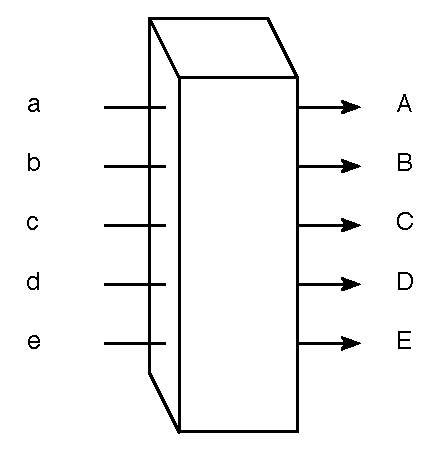
\includegraphics[scale=.6]{media/FA-30/boitenoire5.eps}
%\end{minipage}
%%%%%%%%%%%% FIN BOITES NOIRES EN EPS %%%%%%%%%%%%%%%%%%%%%%%%%%%%%%%%%%%%%%
\begin{center}
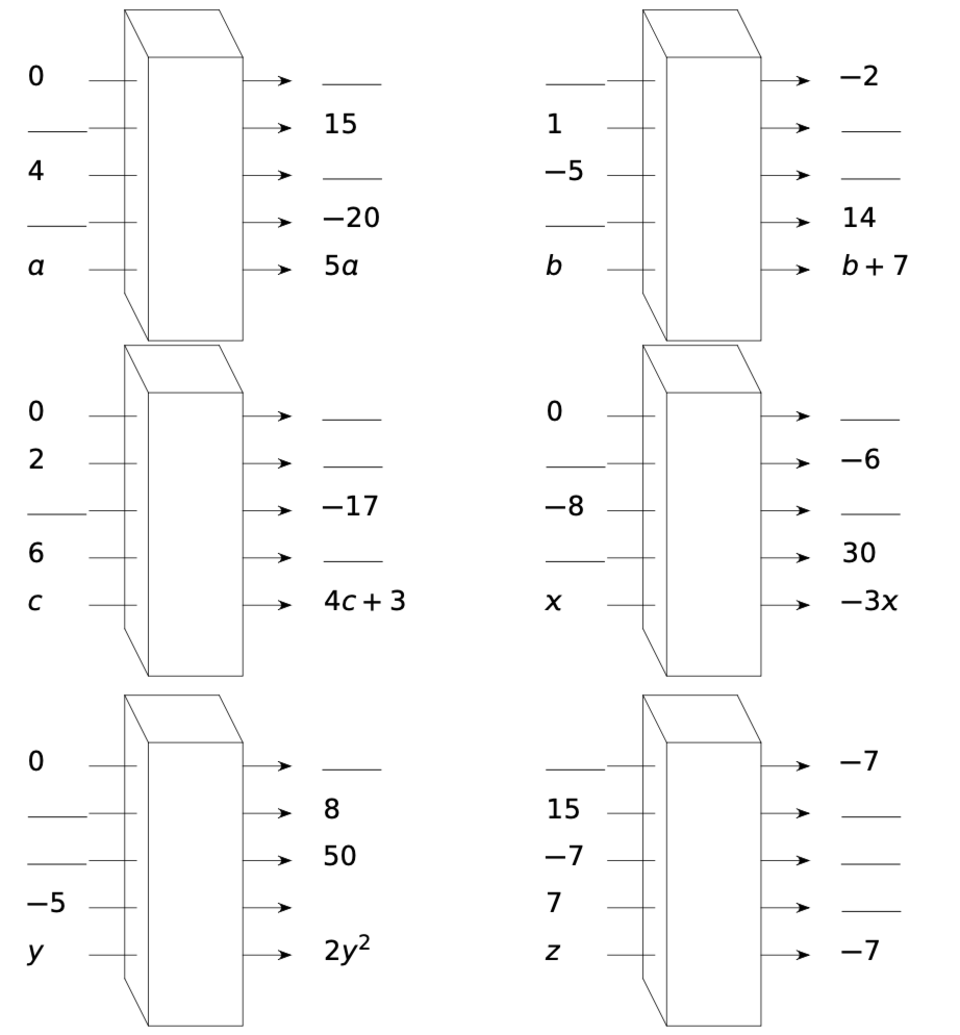
\includegraphics[width=1\textwidth]{media/FA-30/bn11.pdf}
\end{center}

}
{2}

\exof{FA7}{71}{2}
\exof{FA8}{71}{2}


\newpage

\resolu{Vers l'expression fonctionnelle}{Traduis chaque énoncé en français par une expression fonctionnelle.

\begin{center}
{\renewcommand{\arraystretch}{1.8}
\begin{tabular}{|c|p{9cm}|l|}\hline
 & Expression française & Expression fonctionnelle \\\hline
a) &Le double d'un nombre, puis ajouter 4. & $x \mapsto 2x+4$ \\\hline
b) & La moitié d'un nombre puis on retranche 4. & $\displaystyle{x\mapsto\dfrac{x}{2}-4}$ \\\hline
c)& Le carré d'un nombre puis ajouter 1. & $x\mapsto x^2+1$\\\hline
d) & Le carré d'un nombre augmenté de 1. & $x\mapsto (x+1)^2$ \\\hline
e) & Le double du cube d'un nombre. & $x\mapsto 2x^3$\\\hline
f) & Le cube du double d'un nombre. & $x\mapsto (2x)^3$\\\hline
\end{tabular}}
\end{center}}{2}

\newpage

\exop{Traduis chaque énoncé en français par une expression fonctionnelle.

\begin{center}
{\renewcommand{\arraystretch}{1.8}
\begin{tabular}{|c|p{9cm}|l|}\hline
 & Expression française & Expression fonctionnelle \\\hline
a) &Le triple d'un nombre, puis retrancher 3. & $x \mapsto$ \\\hline
b) & Le tiers d'un nombre puis ajouter 10. & $x\mapsto$ \\\hline
c)& Le cube d'un nombre puis retrancher 2. & $x\mapsto$\\\hline
d) & Le cube d'un nombre diminué de 2. & $x\mapsto $ \\\hline
e) & Le quintuple  du carré d'un nombre. & $x\mapsto $\\\hline
f) & Le carré du quintuple d'un nombre. & $x\mapsto $\\\hline
\end{tabular}}
\end{center}
}{2}

\newpage

\exop{Traduis chaque énoncé en français par une expression fonctionnelle.

\begin{center}
{\renewcommand{\arraystretch}{1.8}
\begin{tabular}{|c|p{9cm}|l|}\hline
 & Expression française & Expression fonctionnelle \\\hline
a) & Le double d'un nombre, puis ajouter 7. & $x \mapsto$ \\\hline
b) & Le tiers d'un nombre, ensuite le multiplier par 4. & $x\mapsto$ \\\hline
c)&  Le carré d'un nombre, puis soustraire 6. & $x\mapsto$\\\hline
d) & Le quart d'un nombre, suivi de l'ajout de 3. & $x\mapsto $ \\\hline
e) & La moitié du cube d'un nombre. & $x\mapsto $\\\hline
f) & Le cube de la moitié d'un nombre. & $x\mapsto $\\\hline
\end{tabular}}
\end{center}
}{2}

\newpage

\exop{Traduis chaque énoncé en français par une expression fonctionnelle.
\begin{center}
{\renewcommand{\arraystretch}{1.8}
\begin{tabular}{|c|p{9cm}|l|}\hline
 & Expression française & Expression fonctionnelle \\\hline
a) & Le périmètre d'un triangle équilatéral, dont l'un des côtés mesure $x$ cm. & $x \mapsto$ \\\hline
b) & Le périmètre d'un carré, dont l'un des côtés mesure $x$ cm. & $x\mapsto$ \\\hline
c)&  L'aire d'un carré, dont l'un des côtés mesure $x$ cm. & $x\mapsto$\\\hline
d) & Le volume d'un cube, dont l'une des arêtes mesure $x$ cm. & $x\mapsto $ \\\hline
e) & L'aire totale d'un cube, dont l'une des arêtes mesure $x$ cm. & $x\mapsto $\\\hline
f) & La somme de toutes les arêtes d'un cube, dont l'une des arêtes mesure $x$ cm. & $x\mapsto $\\\hline
\end{tabular}}
\end{center}
}{2}

\exof{FA10}{73}{2}


\newpage

\resolu{Images d'une fonction}{On considère la fonction $f : x \mapsto -3x+2.$

\begin{enumerate}
\item Calcule l'image de 2 par la fonction $f.$

{\bf Réponse : } $f(2)= -3\cdot 2+2 =-6+2 =-4$. Ainsi l'image de 2 par la fonction $f$ est -4 et on la note : $f(2)=-4.$
\item Calcule l'image de 1 par la fonction $f.$

{\bf Réponse : } $f(1)= -3\cdot 1+2 =-3+2 =-1$. Ainsi l'image de 1 par la fonction $f$ est -1 et on la note : $f(1)=-1.$
\item Calcule l'image de 0 par la fonction $f.$

{\bf Réponse : } $f(0)= -3\cdot 0+2 =2$. Ainsi l'image de 0 par la fonction $f$ est 2 et on la note : $f(0)=2.$
\item Calcule l'image de -1 par la fonction $f.$

{\bf Réponse : } $f(-1)= -3\cdot (-1)+2 =+3+2 =5$. Ainsi l'image de -1 par la fonction $f$ est 5 et on la note : $f(-1)=5.$
\item Calcule l'image de -2 par la fonction $f.$

{\bf Réponse : } $f(-2)= -3\cdot (-2)+2 =+6+2 =8$. Ainsi l'image de -2 par la fonction $f$ est 8 et on la note : $f(-2)=8.$
\item En t'aidant de tes calculs précédents, complète le tableau de valeurs ci-dessous pour la fonction $f.$
\begin{center}
$\begin{array}{|c|c|c|c|c|c|}\hline
x&-2&-1&0&+1&+2 \\\hline
f(x)& +8& +5 & +2 &-1 & -4 \\\hline
\end{array}$
\end{center}
\end{enumerate}
}{2}

\exo{On considère la fonction $f : x \mapsto 3x-2.$

\begin{enumerate}
\item Calcule l'image de 2 par la fonction $f.$
\item Calcule l'image de 1 par la fonction $f.$
\item Calcule l'image de 0 par la fonction $f.$
\item Calcule l'image de -1 par la fonction $f.$
\item Calcule l'image de -2 par la fonction $f.$
\item En t'aidant de tes calculs précédents, recopie dans ton cahier et complète le tableau de valeurs ci-dessous pour la fonction $f.$
\begin{center}
{\renewcommand{\arraystretch}{1.5}
$\begin{array}{|c|>{\centering\arraybackslash}p{2cm}|>{\centering\arraybackslash}p{2cm}|>{\centering\arraybackslash}p{2cm}|>{\centering\arraybackslash}p{2cm}|>{\centering\arraybackslash}p{2cm}|}\hline
x&\quad-2 \quad&-1&0&+1&+2 \\\hline
f(x)& &  &  & &  \\\hline
\end{array}$}
\end{center}
\end{enumerate}
}{2}


\exo{On considère la fonction $f : x \mapsto 4x+5.$

\begin{enumerate}
\item Calcule l'image de 2 par la fonction $f.$
\item Calcule l'image de 1 par la fonction $f.$
\item Calcule l'image de 0 par la fonction $f.$
\item Calcule l'image de -1 par la fonction $f.$
\item Calcule l'image de -2 par la fonction $f.$
\item En t'aidant de tes calculs précédents, recopie dans ton cahier et complète le tableau de valeurs ci-dessous pour la fonction $f.$
\begin{center}
{\renewcommand{\arraystretch}{1.5}
$\begin{array}{|c|>{\centering\arraybackslash}p{2cm}|>{\centering\arraybackslash}p{2cm}|>{\centering\arraybackslash}p{2cm}|>{\centering\arraybackslash}p{2cm}|>{\centering\arraybackslash}p{2cm}|}\hline
x&\quad-2 \quad&-1&0&+1&+2 \\\hline
f(x)& &  &  & &  \\\hline
\end{array}$}
\end{center}
\end{enumerate}
}{2}


\resolu{Préimages}{On considère la fonction $f : x \mapsto -2x+1.$
\begin{enumerate}
\item Calcule la ou les préimage(s) de -5 par $f$.

{\bf Réponse :} Pour répondre à cette question on doit résoudre l'équation $f(x)=-5,$ c'est-à-dire qu'on doit résoudre l'équation $-2x+1=-5.$
\begin{center}
$\begin{array}{cccc}
-2x&+1&=&-5\\
&-1& & -1 \\\hline
-2x & & =& -6 \\
:(-2) & & & :(-2) \\\hline
x & & = &  3
\end{array}$
\end{center}
Ainsi la préimage de -5 par $f$ est 3 car $f(3)= -5.$
\item Calcule la ou les préimage(s) de -3 par $f$.

{\bf Réponse :} Pour répondre à cette question on doit résoudre l'équation $f(x)=-3,$ c'est-à-dire qu'on doit résoudre l'équation $-2x+1=-3.$
\begin{center}
$\begin{array}{cccc}
-2x&+1&=&-3\\
&-1& & -1 \\\hline
-2x & & =& -4 \\
:(-2) & & & :(-2) \\\hline
x & & = &  2
\end{array}$
\end{center}
Ainsi la préimage de -3 par $f$ est 2 car $f(2)= -3.$
\item Calcule la ou les préimage(s) de -1 par $f$.

{\bf Réponse :} Pour répondre à cette question on doit résoudre l'équation $f(x)=-1,$ c'est-à-dire qu'on doit résoudre l'équation $-2x+1=-1.$
\begin{center}
$\begin{array}{cccc}
-2x&+1&=&-1\\
&-1& & -1 \\\hline
-2x & & =& -2 \\
:(-2) & & & :(-2) \\\hline
x & & = &  1
\end{array}$
\end{center}
Ainsi la préimage de -1 par $f$ est 1 car $f(1)= -1.$
\item Calcule la ou les préimage(s) de 1 par $f$.

{\bf Réponse :} Pour répondre à cette question on doit résoudre l'équation $f(x)=1,$ c'est-à-dire qu'on doit résoudre l'équation $-2x+1=1.$
\begin{center}
$\begin{array}{cccc}
-2x&+1&=&1\\
&-1& & -1 \\\hline
-2x & & =& 0 \\
:(-2) & & & :(-2) \\\hline
x & & = &  0
\end{array}$
\end{center}
Ainsi la préimage de 1 par $f$ est 0 car $f(0)= 1.$
\item Calcule la ou les préimage(s) de 3 par $f$.

{\bf Réponse :} Pour répondre à cette question on doit résoudre l'équation $f(x)=3,$ c'est-à-dire qu'on doit résoudre l'équation $-2x+1=3.$
\begin{center}
$\begin{array}{cccc}
-2x&+1&=&3\\
&-1& & -1 \\\hline
-2x & & =& 2 \\
:(-2) & & & :(-2) \\\hline
x & & = &  -1
\end{array}$
\end{center}
Ainsi la préimage de 3 par $f$ est -1 car $f(-1)= 3.$
\item Calcule la ou les préimage(s) de 5 par $f$.

{\bf Réponse :} Pour répondre à cette question on doit résoudre l'équation $f(x)=5,$ c'est-à-dire qu'on doit résoudre l'équation $-2x+1=5.$
\begin{center}
$\begin{array}{cccc}
-2x&+1&=&5\\
&-1& & -1 \\\hline
-2x & & =& 4 \\
:(-2) & & & :(-2) \\\hline
x & & = &  -2
\end{array}$
\end{center}
Ainsi la préimage de 5 par $f$ est -2 car $f(-2)= 5.$
\item En t'aidant de tes calculs précédents, complète le tableau de valeurs ci-dessous pour la fonction $f.$
\begin{center}
$\begin{array}{|c|c|c|c|c|c|c|}\hline
x&3 &  2& 1& 0 & -1 & -2 \\\hline 
f(x)& -5&-3&-1&1&3&5 \\\hline
\end{array}$
\end{center}
\end{enumerate}
}{2}

\newpage

\exo{On considère la fonction $f : x \mapsto 2x-1.$
\begin{enumerate}
\item Calcule la ou les préimage(s) de -5 par $f$.
\item Calcule la ou les préimage(s) de -3 par $f$.
\item Calcule la ou les préimage(s) de -1 par $f$.
\item Calcule la ou les préimage(s) de 1 par $f$.
\item Calcule la ou les préimage(s) de 3 par $f$.
\item Calcule la ou les préimage(s) de 5 par $f$.
\item En t'aidant de tes calculs précédents, complète le tableau de valeurs ci-dessous pour la fonction $f.$
\begin{center}
{\renewcommand{\arraystretch}{1.5}
$\begin{array}{|c|>{\centering\arraybackslash}p{2cm}|>{\centering\arraybackslash}p{1.9cm}|>{\centering\arraybackslash}p{1.9cm}|>{\centering\arraybackslash}p{1.9cm}|>{\centering\arraybackslash}p{1.9cm}|>{\centering\arraybackslash}p{1.9cm}|}\hline
x& &  & &  &  &  \\\hline
f(x)& -5&-3&-1&1&3&5 \\\hline
\end{array}$}
\end{center}
\end{enumerate}
}{2}



\exo{On considère la fonction $f : x \mapsto -x-1.$
\begin{enumerate}
\item Calcule la ou les préimage(s) de -9 par $f$.
\item Calcule la ou les préimage(s) de -5 par $f$.
\item Calcule la ou les préimage(s) de -2 par $f$.
\item Calcule la ou les préimage(s) de 0 par $f$.
\item Calcule la ou les préimage(s) de 4 par $f$.
\item Calcule la ou les préimage(s) de 8 par $f$.
\item En t'aidant de tes calculs précédents, recopie dans ton cahier et complète le tableau de valeurs ci-dessous pour la fonction $f.$
\begin{center}
{\renewcommand{\arraystretch}{1.5}
$\begin{array}{|c|>{\centering\arraybackslash}p{2cm}|>{\centering\arraybackslash}p{1.9cm}|>{\centering\arraybackslash}p{1.9cm}|>{\centering\arraybackslash}p{1.9cm}|>{\centering\arraybackslash}p{1.9cm}|>{\centering\arraybackslash}p{1.9cm}|}\hline
x& &  & &  &  &  \\\hline
f(x)& -9&-5&-2&0&4&8 \\\hline
\end{array}$}
\end{center}
\end{enumerate}
}{2}


\exo{On considère la fonction $f : x \mapsto x+8.$
\begin{enumerate}
\item Calcule la ou les préimage(s) de -12 par $f$.
\item Calcule la ou les préimage(s) de -7 par $f$.
\item Calcule la ou les préimage(s) de -1 par $f$.
\item Calcule la ou les préimage(s) de 0 par $f$.
\item Calcule la ou les préimage(s) de 5 par $f$.
\item Calcule la ou les préimage(s) de 11 par $f$.
\item En t'aidant de tes calculs précédents, recopie dans ton cahier et complète le tableau de valeurs ci-dessous pour la fonction $f.$
\begin{center}
{\renewcommand{\arraystretch}{1.5}
$\begin{array}{|c|>{\centering\arraybackslash}p{2cm}|>{\centering\arraybackslash}p{1.9cm}|>{\centering\arraybackslash}p{1.9cm}|>{\centering\arraybackslash}p{1.9cm}|>{\centering\arraybackslash}p{1.9cm}|>{\centering\arraybackslash}p{1.9cm}|}\hline
x& &  & &  &  &  \\\hline
f(x)& -12&-7&-1&0&5&11 \\\hline
\end{array}$}
\end{center}
\end{enumerate}
}{2}

\exop{\begin{enumerate}
\item Considérons la fonction $f : x \mapsto 3x$. Complète le tableau de valeurs suivants :

\medskip

{\renewcommand{\arraystretch}{1.5}\setlength{\tabcolsep}{.4cm}
\begin{tabular}{|c|c|c|c|c|c|c|c|c|c|c|}\hline
x & -10 & -5 & -3 & -1 & 0 & 1 & 3 & 5 & 8 & 12\\\hline
f(x) & & & & & & & & & & \\\hline
\end{tabular}}
\item Considérons la fonction $g : x \mapsto 2x+4$. Complète le tableau de valeurs suivants :

\medskip

{\renewcommand{\arraystretch}{1.5}\setlength{\tabcolsep}{.4cm}
\begin{tabular}{|c|c|c|c|c|c|c|c|c|c|c|}\hline
x & -7 & -4 & -2 & -1 & 0 & 1 & 4 & 6 & 9 & 11\\\hline
g(x) & & & & & & & & & & \\\hline
\end{tabular}}

\item Considérons la fonction $h : x \mapsto -4$. Complète le tableau de valeurs suivants :

\medskip

{\renewcommand{\arraystretch}{1.5}\setlength{\tabcolsep}{.4cm}
\begin{tabular}{|c|c|c|c|c|c|c|c|c|c|c|}\hline
x & -7 & -4 & -2 & -1 & 0 & 1 & 4 & 6 & 9 & 11\\\hline
h(x) & & & & & & & & & & \\\hline
\end{tabular}}

\item Considérons la fonction $i : x \mapsto x^2$. Complète le tableau de valeurs suivants :

\medskip

{\renewcommand{\arraystretch}{1.5}\setlength{\tabcolsep}{.4cm}
\begin{tabular}{|c|c|c|c|c|c|c|c|c|c|c|}\hline
x & -6 & -4 & -3 & -2 & 0 & 1 & 3 & 5 & 7 & 10\\\hline
i(x) & & & & & & & & & & \\\hline
\end{tabular}}

\item Considérons la fonction $j : x \mapsto -x^2$. Complète le tableau de valeurs suivants :

\medskip

{\renewcommand{\arraystretch}{1.5}\setlength{\tabcolsep}{.4cm}
\begin{tabular}{|c|c|c|c|c|c|c|c|c|c|c|}\hline
x & -5 & -4 & -3 & -2 & -1 & 0 & 1 & 2 & 3 & 12\\\hline
j(x) & & & & & & & & & & \\\hline
\end{tabular}}

\end{enumerate}
}{2}


\exop{\begin{enumerate}
\item Considérons la fonction $f : x \mapsto -3x$. Complète le tableau de valeurs suivants :

\medskip

{\renewcommand{\arraystretch}{1.5}\setlength{\tabcolsep}{.4cm}
\begin{tabular}{|c|c|c|c|c|c|c|c|c|c|c|}\hline
x 		& -10 	&  	&  	& -1 	& 0 	&  	&  	& 5 	& 8	& \\\hline
f(x) 	& 			& 	21	& 	12	& 			& 		& 	-6	& 	-12	& 		& 		&-36 \\\hline
\end{tabular}}
\item Considérons la fonction $g : x \mapsto 2x+2$. Complète le tableau de valeurs suivants :

\medskip

{\renewcommand{\arraystretch}{1.5}\setlength{\tabcolsep}{.4cm}
\begin{tabular}{|c|c|c|c|c|c|c|c|c|c|c|}\hline
x 		&  		&  		& -2 & -1 & 0 & 1 	& 4 	&  	&  	& \\\hline
g(x) & -10	& -6		& 		& 		& 		& 		& 		& 14		& 	20	& 24 \\\hline
\end{tabular}}

\item Considérons la fonction $h : x \mapsto 3$. Complète le tableau de valeurs suivants :

\medskip

{\renewcommand{\arraystretch}{1.5}\setlength{\tabcolsep}{.4cm}
\begin{tabular}{|c|c|c|c|c|c|c|c|c|c|c|}\hline
x & -8 & -5 & -3 & -1 & 0 & 1 & 5 & 7 & 9 & 15\\\hline
h(x) & & & & & & & & & & \\\hline
\end{tabular}}

\item Considérons la fonction $i : x \mapsto 2x^2$. Complète le tableau de valeurs suivants :

\medskip

{\renewcommand{\arraystretch}{1.5}\setlength{\tabcolsep}{.4cm}
\begin{tabular}{|c|c|c|c|c|c|c|c|c|c|c|}\hline
x & -10 & -8 & -4 & -2 & 0 & 1 & 3 & 5 & 7 & 9\\\hline
i(x) & & & & & & & & & & \\\hline
\end{tabular}}

\item Considérons la fonction $j : x \mapsto -2x^2$. Complète le tableau de valeurs suivants :

\medskip

{\renewcommand{\arraystretch}{1.5}\setlength{\tabcolsep}{.4cm}
\begin{tabular}{|c|c|c|c|c|c|c|c|c|c|c|}\hline
x & -10 & -8 & -4 & -2 & -1 & 0 & 1 & 3 & 5 & 7\\\hline
j(x) & & & & & & & & & & \\\hline
\end{tabular}}

\end{enumerate}
}{2}

\newpage

\resolu{Placer des points}{
\begin{enumerate}
\item Place les points suivants sur le système d'axes ci-dessous :
\begin{center}
$A(0;-2) \qquad B(5;3)\qquad C(-3;-5)\qquad D(2;0) \qquad E(-2;-4)$

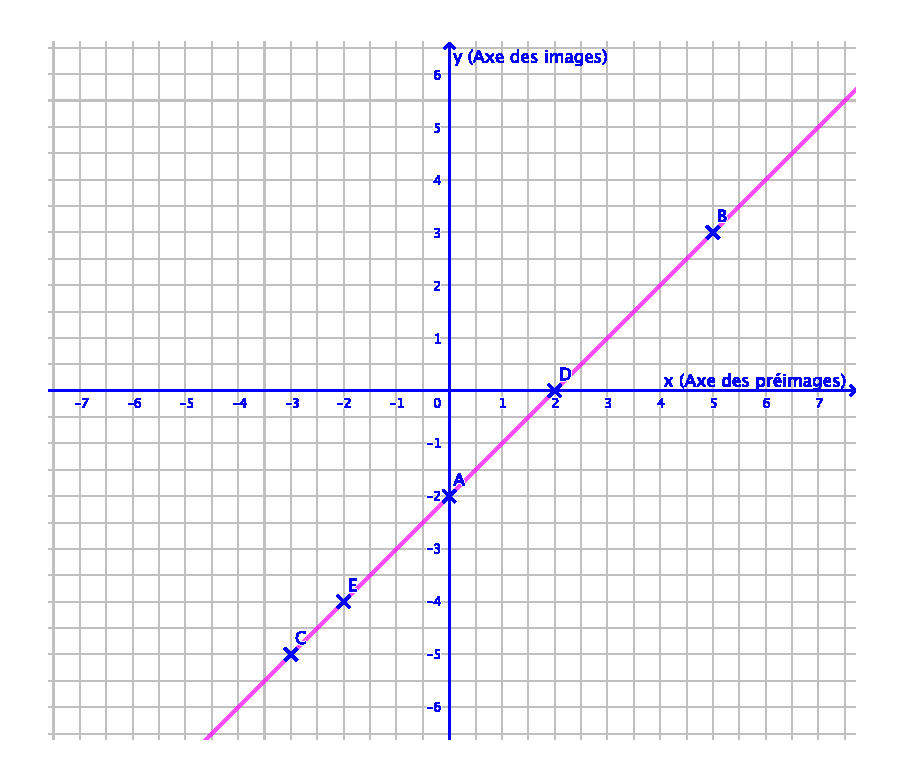
\includegraphics[width=1\textwidth]{media/FA-30/axesABCDE.pdf}
\end{center}
\item On considère la fonction $f: x \mapsto x-2.$ Complète le tableau de valeurs ci-dessous :

\begin{center}
{\renewcommand{\arraystretch}{1.5}\setlength{\tabcolsep}{.4cm}
\begin{tabular}{|c|c|c|c|c|c|}\hline
x& 0 & 5&-3&2&-2 \\\hline
f(x)&-2&3&-5&0&-4\\\hline
\end{tabular}}
\end{center}
\item Qu'observes-tu ? Quel lien existe-t-il entre les question a et b ?

{\bf Réponse :} Les points $A, B, C, D$ et $E$ sont alignés. On observe également que chaque couple de coordonnées des points $A, B, C, D$ et $E$ correspond à un couple du tableau de valeurs. La représentation graphique d'une fonction $f$ est la courbe constituée de l'ensemble des points de coordonnées $\left(x ; f(x)\right).$ Par convention, l'axe des abscisses (axe des préimages) se lit horizontalement et l'axe des ordonnées (axe des images) se lit verticalement.
\end{enumerate} 

}{2}

\newpage

\exop{
\begin{enumerate}
\item Place les points suivants sur le système d'axe ci-dessous :
\begin{center}
$A(0;2) \qquad B(5;-3)\qquad C(-3;5)\qquad D(2;0) \qquad E(-2;4)$

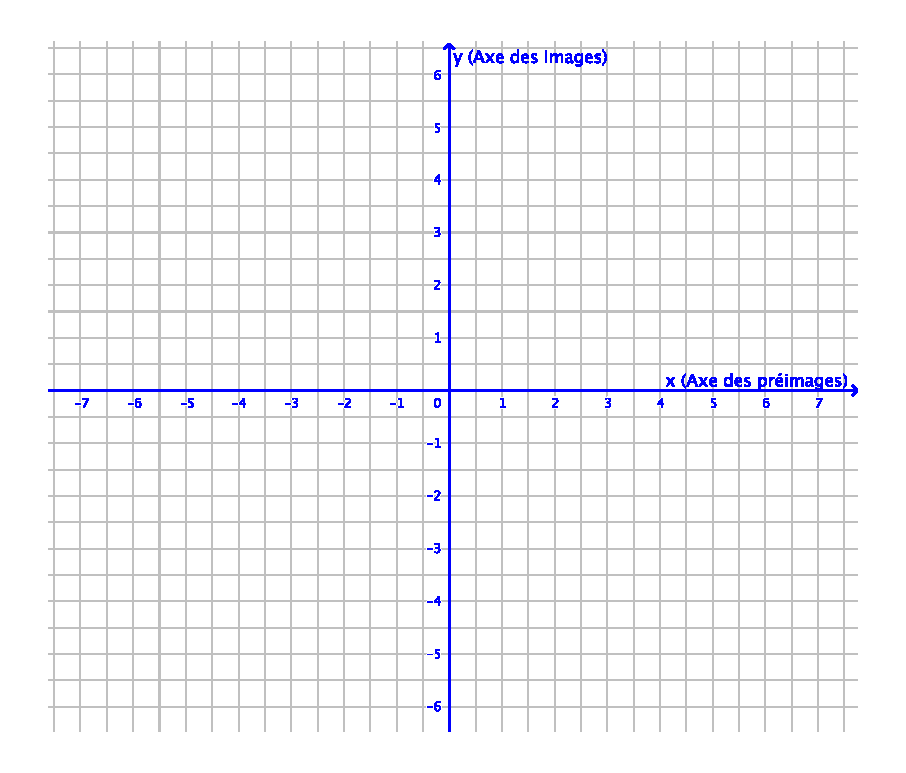
\includegraphics[width=1\textwidth]{media/FA-30/axesvides.pdf}
\end{center}
\item On considère la fonction $f: x \mapsto -x+2.$ Complète le tableau de valeurs ci-dessous :

\begin{center}
{\renewcommand{\arraystretch}{1.5}\setlength{\tabcolsep}{.4cm}
\begin{tabular}{|c|c|c|c|c|c|}\hline
x& 0 & &-3&&-2 \\\hline
f(x)&&-3& &0& \\\hline
\end{tabular}}
\end{center}
\item Qu'observes-tu ? Quel lien existe-t-il entre les question a et b ?
\end{enumerate} 

}{2}

\newpage

\exo{\begin{enumerate}

\item Considérons la fonction $g : x \mapsto 2x+2$. Recopie dans ton cahier et complète le tableau de valeurs suivants :


\medskip

{\renewcommand{\arraystretch}{1.5}\setlength{\tabcolsep}{.4cm}
\begin{tabular}{|c|c|c|c|c|c|c|c|c|c|c|}\hline
x & -5 & -4 & -3 & -2 & -1 & 0 & 1 & 2 & 3 & 4\\\hline
f(x) & & & & & & & & & & \\\hline
\end{tabular}}
\item Construis un système d'axes dans ton cahier (ou utilise l'un des systèmes d'axes en annexe) et place les points obtenus précédemment. Qu'observes-tu ?

%\begin{center}
%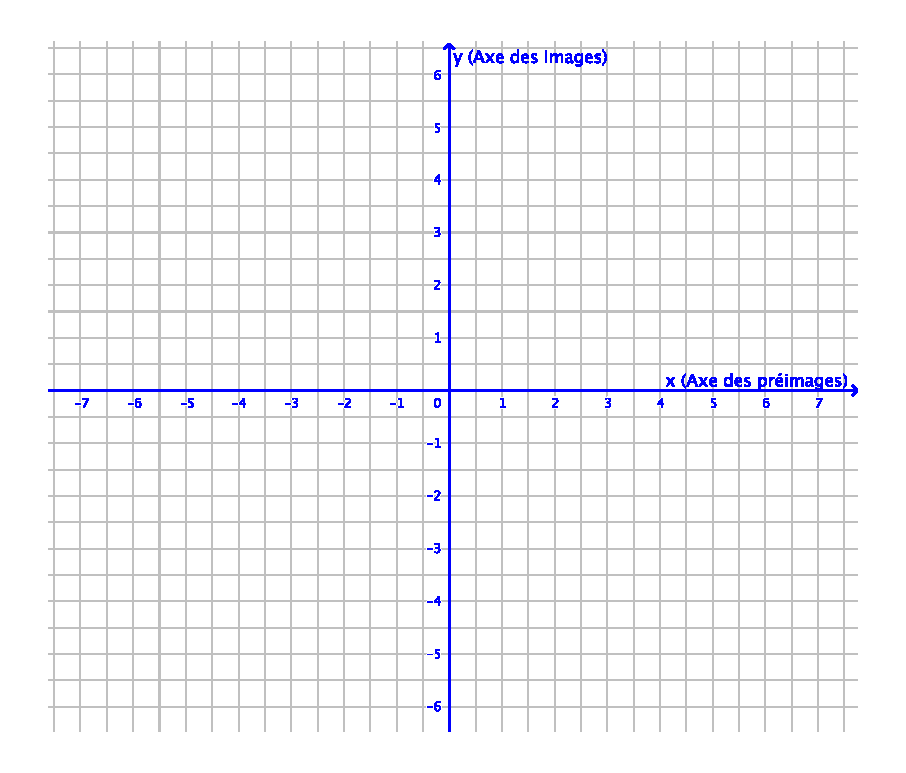
\includegraphics[width=1\textwidth]{media/FA-30/axesvides.pdf}
%\end{center}


\end{enumerate}
}{2}






\exo{
\begin{enumerate}

\item Considérons la fonction $f : x \mapsto x$.  Recopie dans ton cahier et complète le tableau de valeurs suivants :


\medskip

{\renewcommand{\arraystretch}{1.5}\setlength{\tabcolsep}{.4cm}
\begin{tabular}{|c|c|c|c|c|c|c|c|c|c|c|}\hline
x & -5 & -4 & -3 & -2 & -1 & 0 & 1 & 2 & 3 & 4\\\hline
f(x) & & & & & & & & & & \\\hline
\end{tabular}}
\item Construis un système d'axes dans ton cahier (ou utilise l'un des systèmes d'axes en annexe) et place les points obtenus précédemment. Qu'observes-tu ?

%\begin{center}
%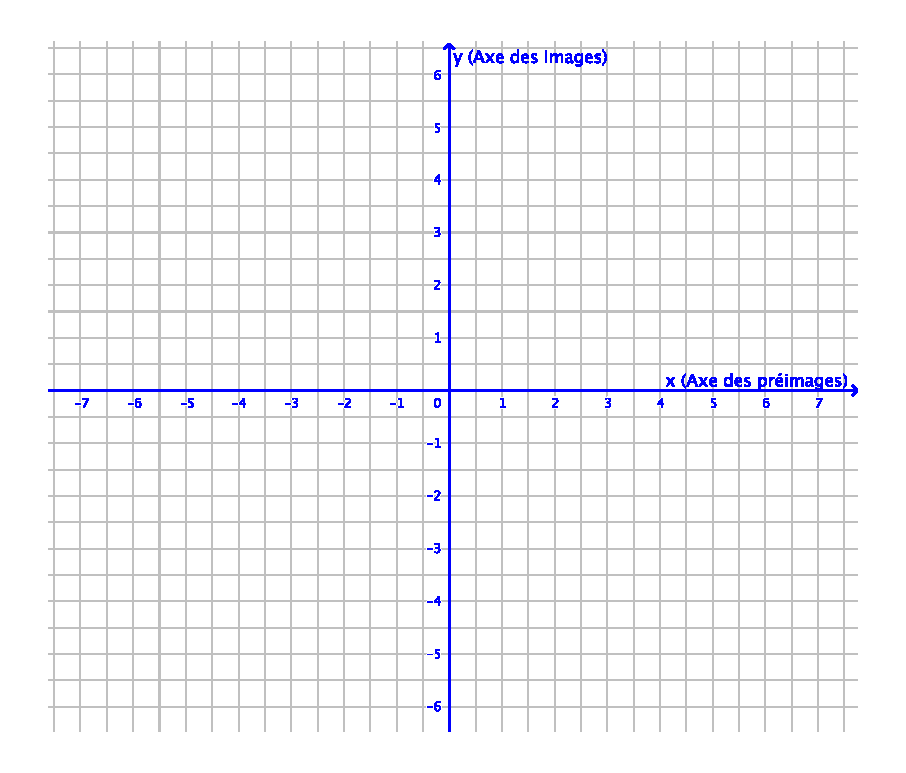
\includegraphics[width=1\textwidth]{media/FA-30/axesvides.pdf}
%\end{center}

\end{enumerate}
}{2}

\exo{
\begin{enumerate}

\item Considérons la fonction $f : x \mapsto -x$.  Recopie dans ton cahier et complète le tableau de valeurs suivants :


\medskip

{\renewcommand{\arraystretch}{1.5}\setlength{\tabcolsep}{.4cm}
\begin{tabular}{|c|c|c|c|c|c|c|c|c|c|c|}\hline
x & -5 & -4 & -3 & -2 & -1 & 0 & 1 & 2 & 3 & 4\\\hline
f(x) & & & & & & & & & & \\\hline
\end{tabular}}
\item Construis un système d'axes dans ton cahier (ou utilise l'un des systèmes d'axes en annexe) et place les points obtenus précédemment. Qu'observes-tu ?

%\begin{center}
%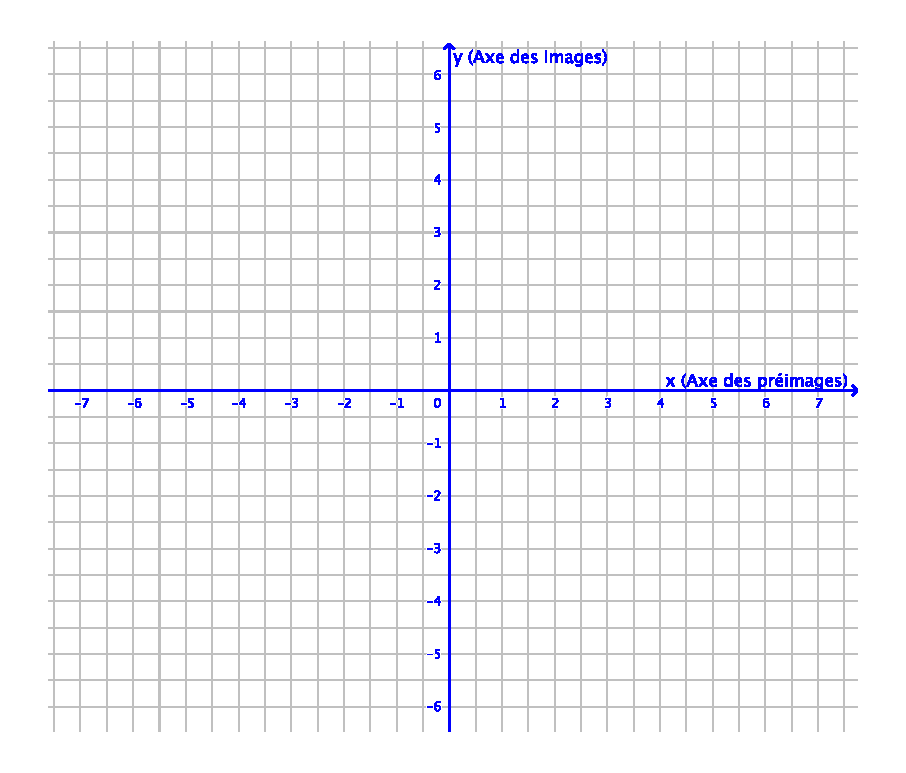
\includegraphics[width=1\textwidth]{media/FA-30/axesvides.pdf}
%\end{center}


\end{enumerate}
}{2}

\exo{
\begin{enumerate}

\item Considérons la fonction $f : x \mapsto x+2$.  Recopie dans ton cahier et complète le tableau de valeurs suivants :


\medskip

{\renewcommand{\arraystretch}{1.5}\setlength{\tabcolsep}{.4cm}
\begin{tabular}{|c|c|c|c|c|c|c|c|c|c|c|}\hline
x & -5 & -4 & -3 & -2 & -1 & 0 & 1 & 2 & 3 & 4\\\hline
f(x) & & & & & & & & & & \\\hline
\end{tabular}}
\item Construis un système d'axes dans ton cahier (ou utilise l'un des systèmes d'axes en annexe) et place les points obtenus précédemment. Qu'observes-tu ?

%\begin{center}
%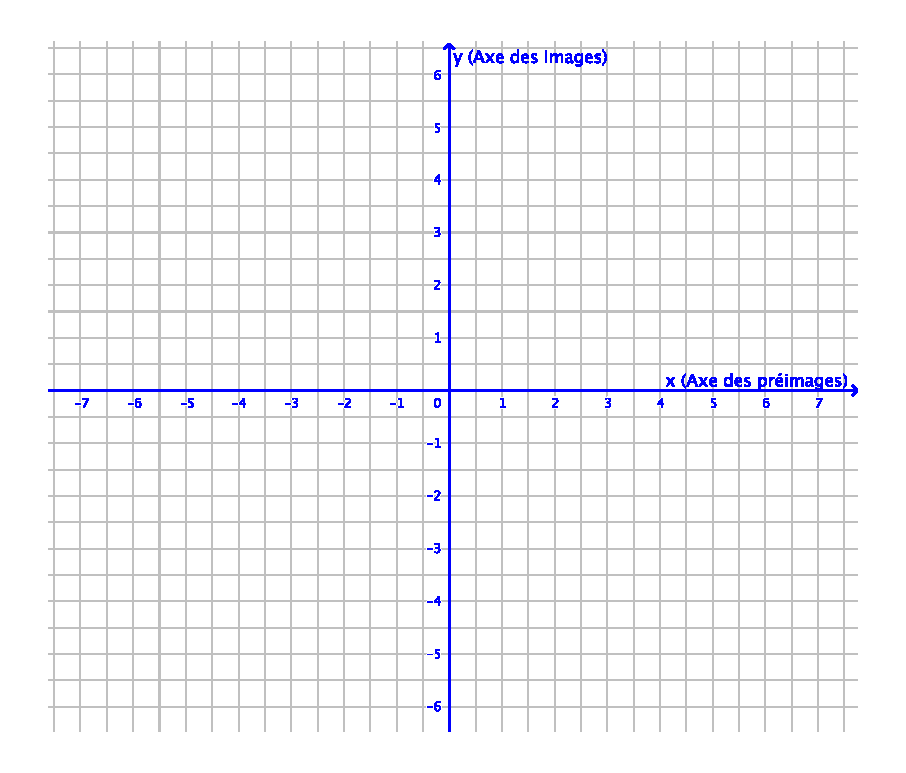
\includegraphics[width=1\textwidth]{media/FA-30/axesvides.pdf}
%\end{center}

\end{enumerate}
}{2} 

\exo{
\begin{enumerate}

\item Considérons la fonction $f : x \mapsto x-5$. Recopie dans ton cahier et complète le tableau de valeurs suivants :


\medskip

{\renewcommand{\arraystretch}{1.5}\setlength{\tabcolsep}{.4cm}
\begin{tabular}{|c|c|c|c|c|c|c|c|c|c|c|}\hline
x & -5 & -4 & -3 & -2 & -1 & 0 & 1 & 2 & 3 & 4\\\hline
f(x) & & & & & & & & & & \\\hline
\end{tabular}}
\item Construis un système d'axes dans ton cahier (ou utilise l'un des systèmes d'axes en annexe) et place les points obtenus précédemment. Qu'observes-tu ?

%\begin{center}
%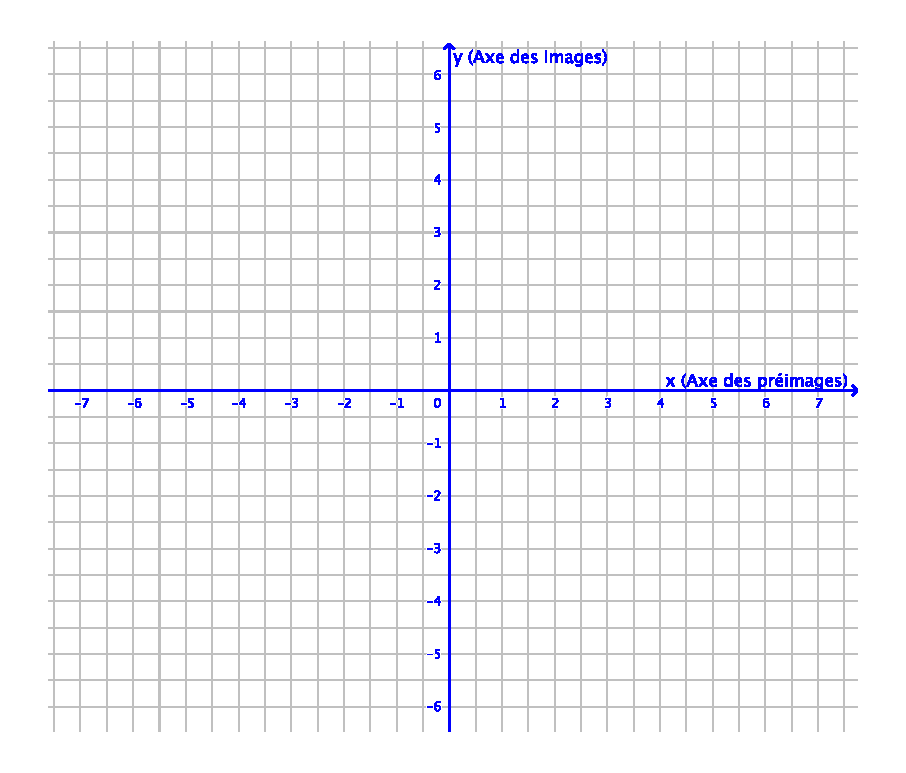
\includegraphics[width=1\textwidth]{media/FA-30/axesvides.pdf}
%\end{center}

\end{enumerate}
}{2}

\exo{
\begin{enumerate}

\item Considérons la fonction $f : x \mapsto -x+3$. Recopie dans ton cahier et complète le tableau de valeurs suivants :


\medskip

{\renewcommand{\arraystretch}{1.5}\setlength{\tabcolsep}{.4cm}
\begin{tabular}{|c|c|c|c|c|c|c|c|c|c|c|}\hline
x & -5 & -4 & -3 & -2 & -1 & 0 & 1 & 2 & 3 & 4\\\hline
f(x) & & & & & & & & & & \\\hline
\end{tabular}}
\item Construis un système d'axes dans ton cahier (ou utilise l'un des systèmes d'axes en annexe) et place les points obtenus précédemment. Qu'observes-tu ?

%\begin{center}
%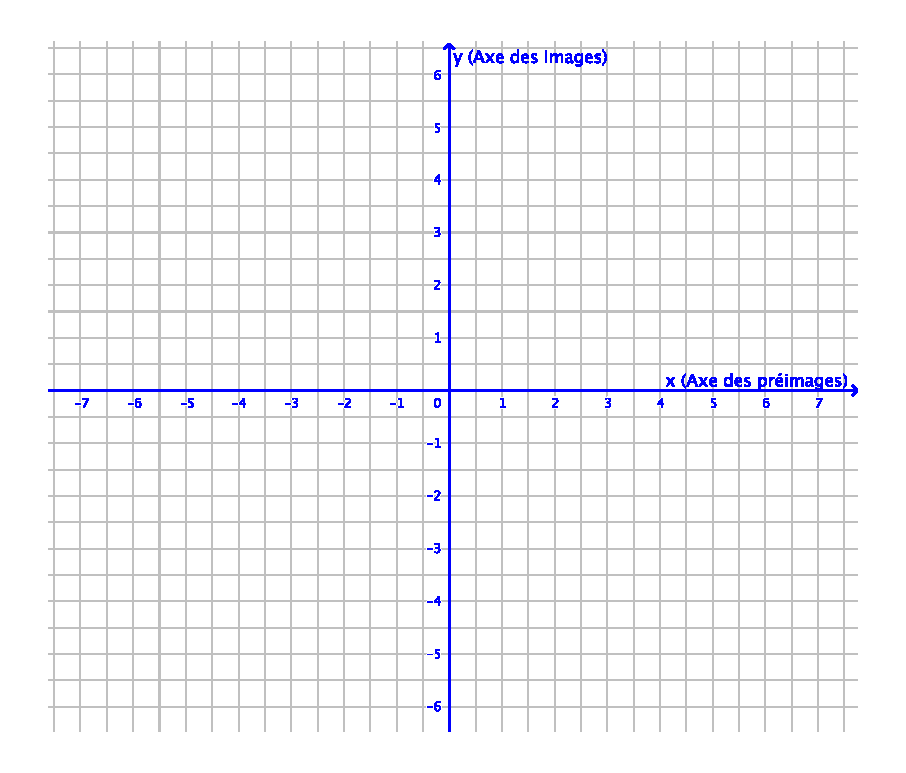
\includegraphics[width=1\textwidth]{media/FA-30/axesvides.pdf}
%\end{center}


\end{enumerate}
}{2}

\exo{
\begin{enumerate}

\item Considérons la fonction $f : x \mapsto 2x$. Recopie dans ton cahier et complète le tableau de valeurs suivants :


\medskip

{\renewcommand{\arraystretch}{1.5}\setlength{\tabcolsep}{.4cm}
\begin{tabular}{|c|c|c|c|c|c|c|c|c|c|c|}\hline
x & -5 & -4 & -3 & -2 & -1 & 0 & 1 & 2 & 3 & 4\\\hline
f(x) & & & & & & & & & & \\\hline
\end{tabular}}
\item Construis un système d'axes dans ton cahier (ou utilise l'un des systèmes d'axes en annexe) et place les points obtenus précédemment. Qu'observes-tu ?

%\begin{center}
%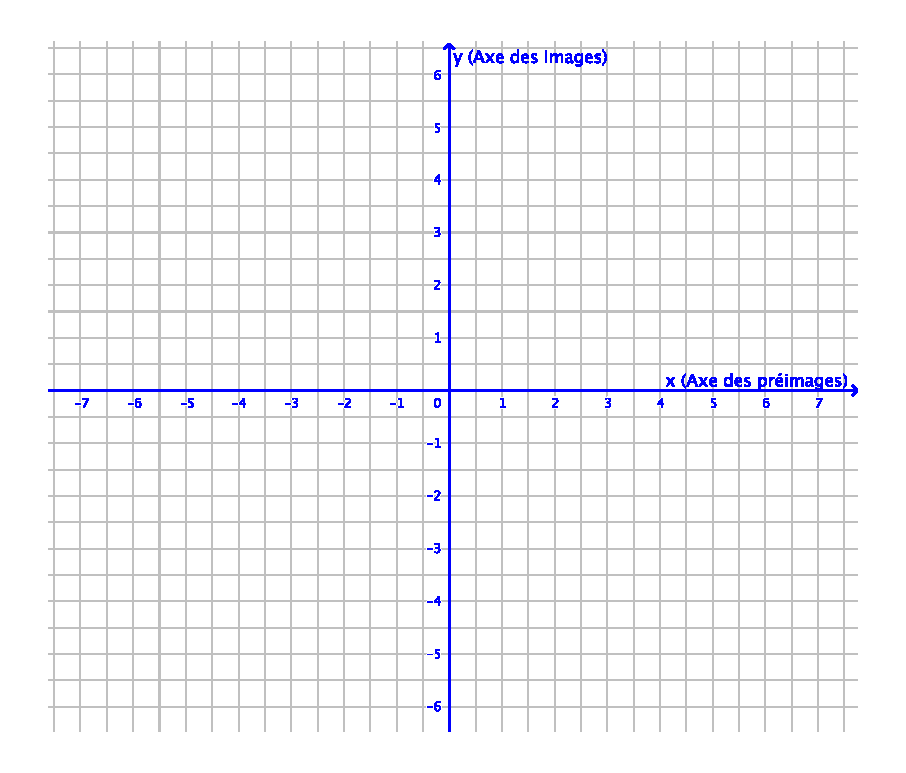
\includegraphics[width=1\textwidth]{media/FA-30/axesvides.pdf}
%\end{center}

\end{enumerate}

}{2}

\exo{
\begin{enumerate}

\item Considérons la fonction $f : x \mapsto -2x$. Recopie dans ton cahier et complète le tableau de valeurs suivants :


\medskip

{\renewcommand{\arraystretch}{1.5}\setlength{\tabcolsep}{.4cm}
\begin{tabular}{|c|c|c|c|c|c|c|c|c|c|c|}\hline
x & -5 & -4 & -3 & -2 & -1 & 0 & 1 & 2 & 3 & 4\\\hline
f(x) & & & & & & & & & & \\\hline
\end{tabular}}
\item Construis un système d'axes dans ton cahier (ou utilise l'un des systèmes d'axes en annexe) et place les points obtenus précédemment. Qu'observes-tu ?

%\begin{center}
%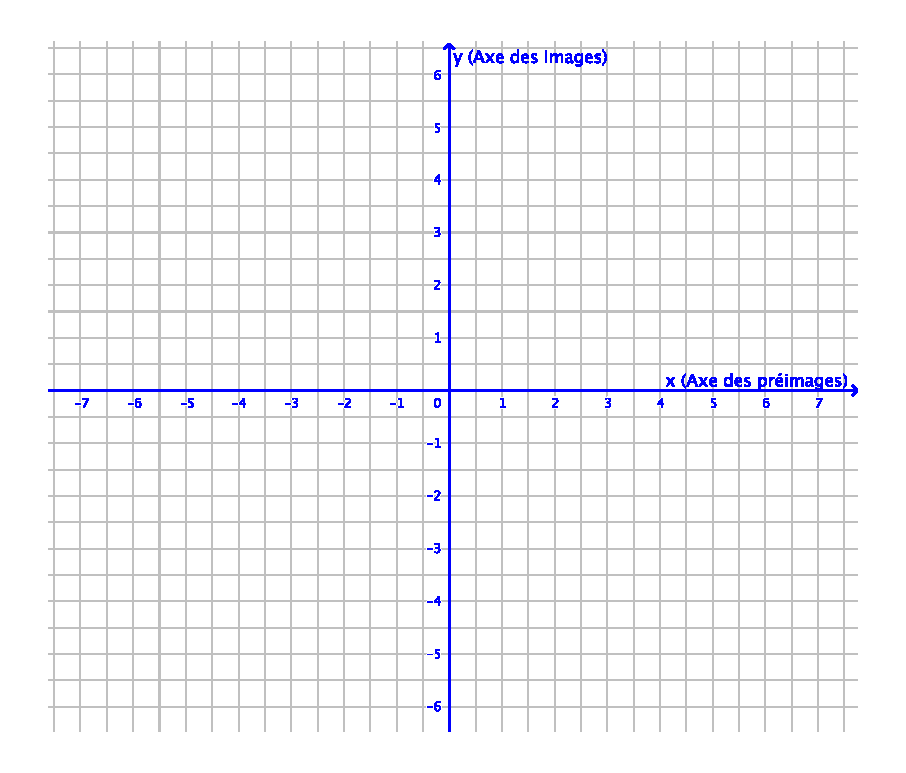
\includegraphics[width=1\textwidth]{media/FA-30/axesvides.pdf}
%\end{center}


\end{enumerate}
}{2}

\exo{
\begin{enumerate}

\item Considérons la fonction $f : x \mapsto -2x+1$. Recopie dans ton cahier et complète le tableau de valeurs suivants :


\medskip

{\renewcommand{\arraystretch}{1.5}\setlength{\tabcolsep}{.4cm}
\begin{tabular}{|c|c|c|c|c|c|c|c|c|c|c|}\hline
x & -5 & -4 & -3 & -2 & -1 & 0 & 1 & 2 & 3 & 4\\\hline
f(x) & & & & & & & & & & \\\hline
\end{tabular}}
\item Construis un système d'axes dans ton cahier (ou utilise l'un des systèmes d'axes en annexe) et place les points obtenus précédemment. Qu'observes-tu ?

%\begin{center}
%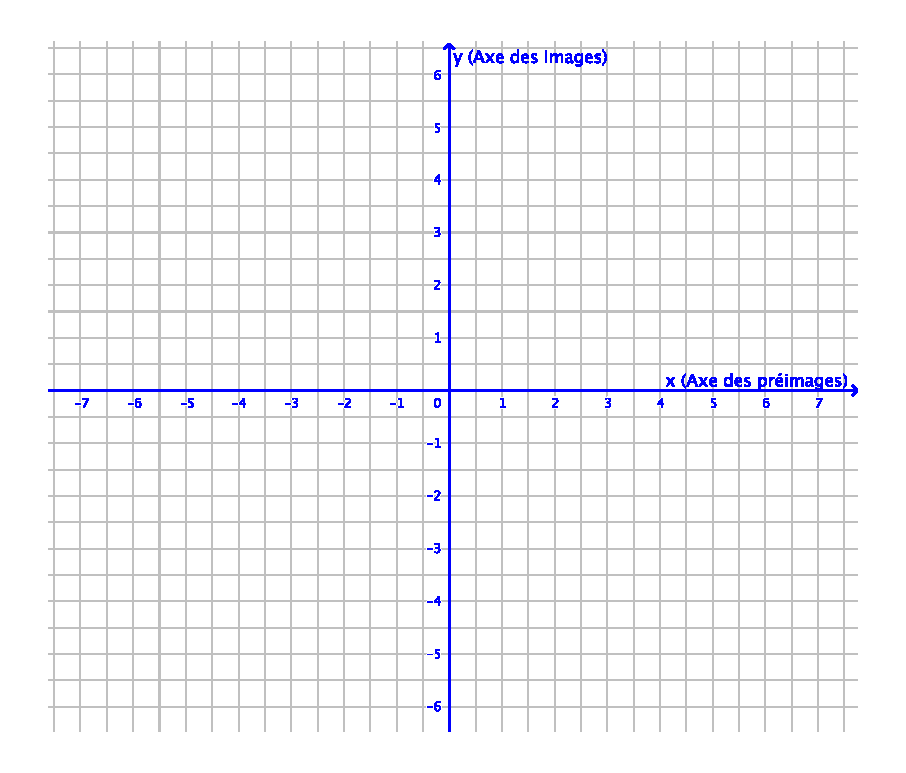
\includegraphics[width=1\textwidth]{media/FA-30/axesvides.pdf}
%\end{center}


\end{enumerate}
}{2}

\exo{
\begin{enumerate}

\item Considérons la fonction $f : x \mapsto 2x-3$. Recopie dans ton cahier et complète le tableau de valeurs suivants :


\medskip

{\renewcommand{\arraystretch}{1.5}\setlength{\tabcolsep}{.4cm}
\begin{tabular}{|c|c|c|c|c|c|c|c|c|c|c|}\hline
x & -5 & -4 & -3 & -2 & -1 & 0 & 1 & 2 & 3 & 4\\\hline
f(x) & & & & & & & & & & \\\hline
\end{tabular}}
\item Construis un système d'axes dans ton cahier (ou utilise l'un des systèmes d'axes en annexe) et place les points obtenus précédemment. Qu'observes-tu ?

%\begin{center}
%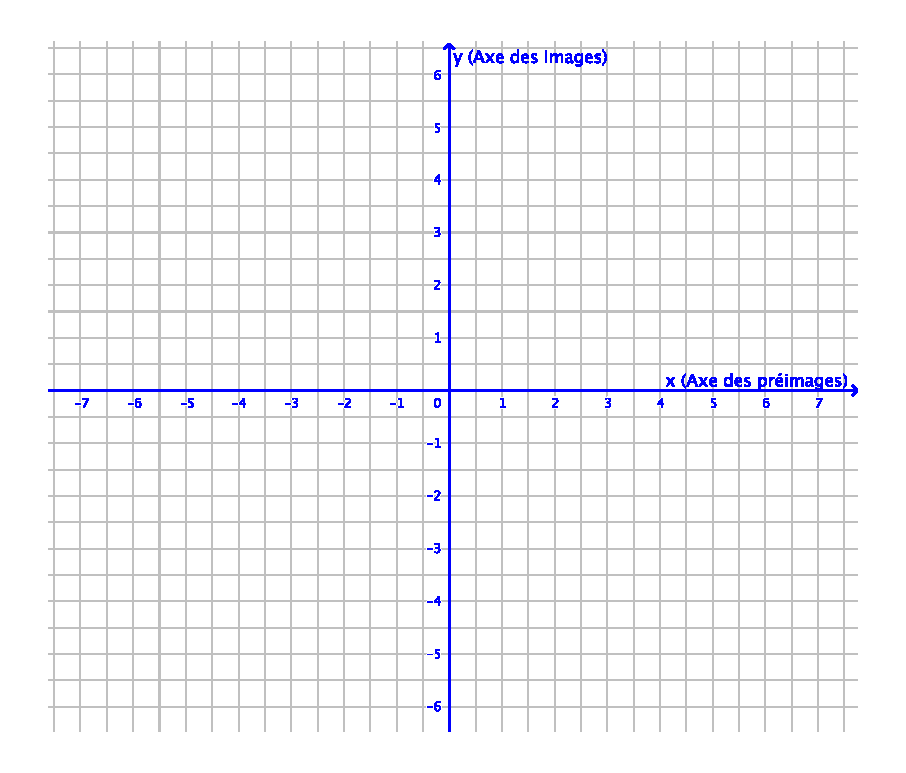
\includegraphics[width=1\textwidth]{media/FA-30/axesvides.pdf}
%\end{center}
\end{enumerate}

}{2}

\exo{
\begin{enumerate}

\item Considérons la fonction $f : x \mapsto -3$. Recopie dans ton cahier et complète le tableau de valeurs suivants :


\medskip

{\renewcommand{\arraystretch}{1.5}\setlength{\tabcolsep}{.4cm}
\begin{tabular}{|c|c|c|c|c|c|c|c|c|c|c|}\hline
x & -5 & -4 & -3 & -2 & -1 & 0 & 1 & 2 & 3 & 4\\\hline
f(x) & & & & & & & & & & \\\hline
\end{tabular}}
\item Construis un système d'axes dans ton cahier (ou utilise l'un des systèmes d'axes en annexe) et place les points obtenus précédemment. Qu'observes-tu ?

%\begin{center}
%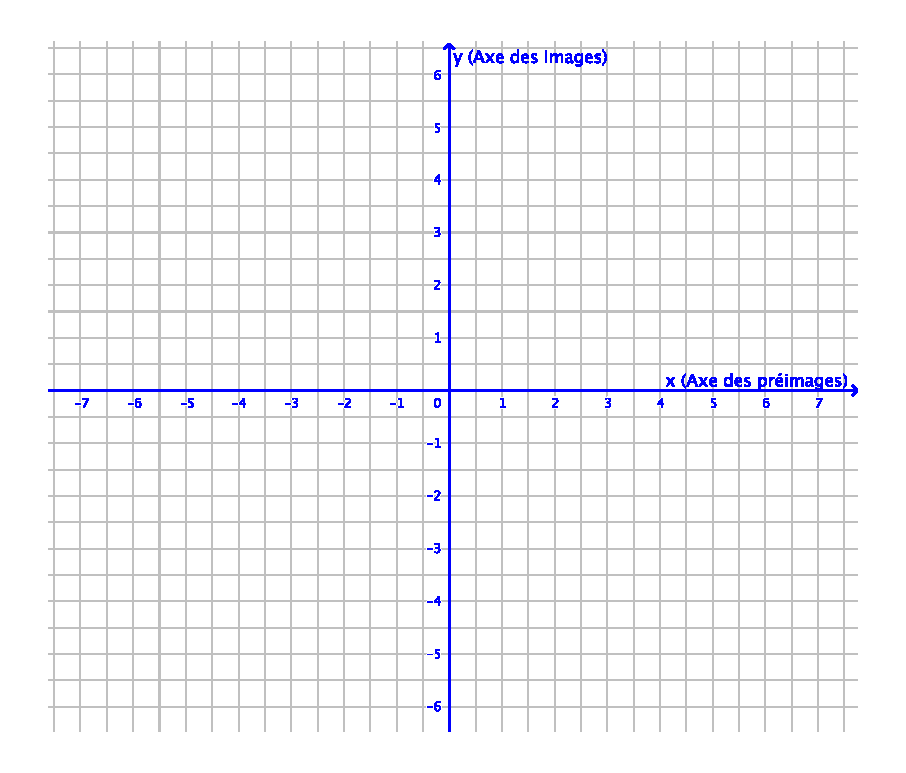
\includegraphics[width=1\textwidth]{media/FA-30/axesvides.pdf}
%\end{center}


\end{enumerate}
}{2}

\exo{
\begin{enumerate}

\item Considérons la fonction $f : x \mapsto +5$. Recopie dans ton cahier et complète le tableau de valeurs suivants :


\medskip

{\renewcommand{\arraystretch}{1.5}\setlength{\tabcolsep}{.4cm}
\begin{tabular}{|c|c|c|c|c|c|c|c|c|c|c|}\hline
x & -5 & -4 & -3 & -2 & -1 & 0 & 1 & 2 & 3 & 4\\\hline
f(x) & & & & & & & & & & \\\hline
\end{tabular}}
\item Construis un système d'axes dans ton cahier (ou utilise l'un des systèmes d'axes en annexe) et place les points obtenus précédemment. Qu'observes-tu ?

%\begin{center}
%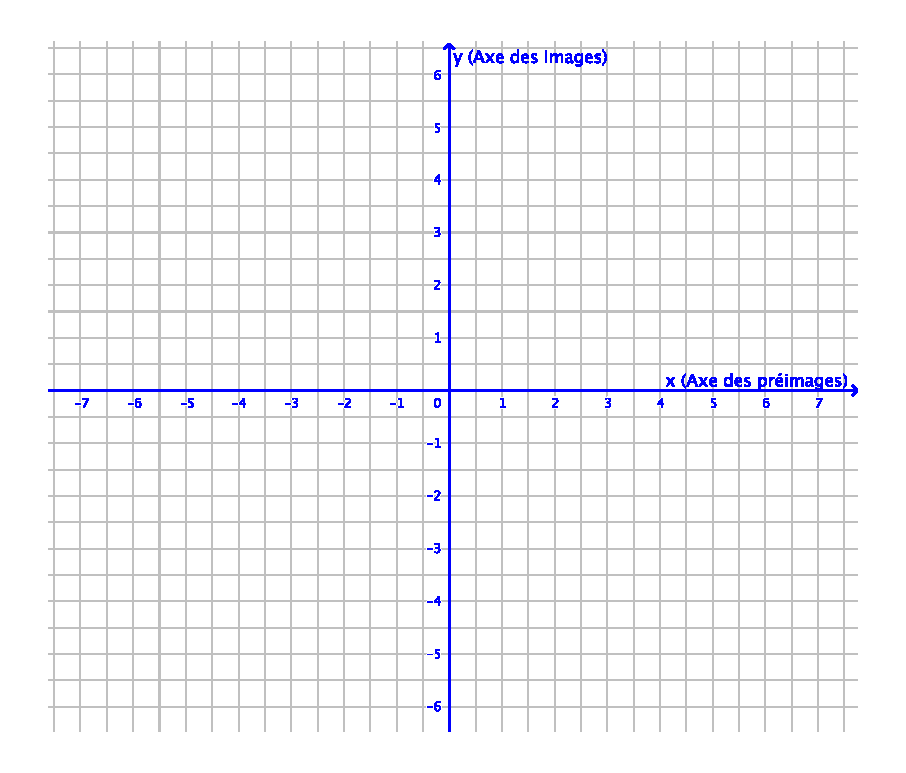
\includegraphics[width=1\textwidth]{media/FA-30/axesvides.pdf}
%\end{center}


\end{enumerate}
}{2}

\exo{
\begin{enumerate}

\item Considérons la fonction $f : x \mapsto 0$. Recopie dans ton cahier et complète le tableau de valeurs suivants :


\medskip

{\renewcommand{\arraystretch}{1.5}\setlength{\tabcolsep}{.4cm}
\begin{tabular}{|c|c|c|c|c|c|c|c|c|c|c|}\hline
x & -5 & -4 & -3 & -2 & -1 & 0 & 1 & 2 & 3 & 4\\\hline
f(x) & & & & & & & & & & \\\hline
\end{tabular}}
\item Construis un système d'axes dans ton cahier (ou utilise l'un des systèmes d'axes en annexe) et place les points obtenus précédemment. Qu'observes-tu ?

%\begin{center}
%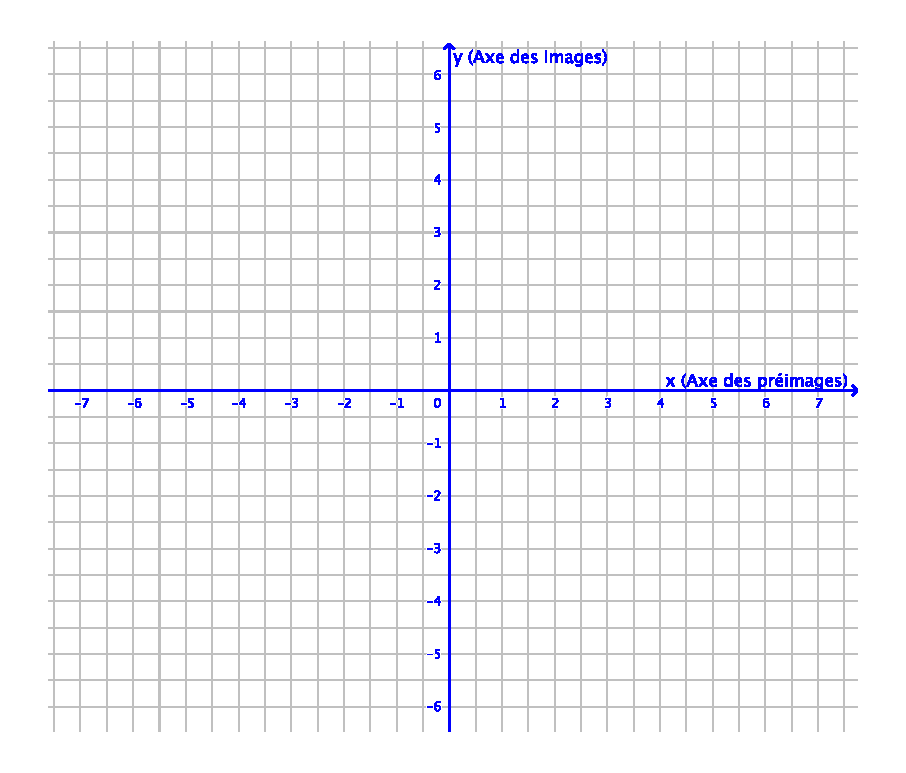
\includegraphics[width=1\textwidth]{media/FA-30/axesvides.pdf}
%\end{center}


\end{enumerate}
}{2}

\exo{
\begin{enumerate}

\item Considérons la fonction $f : x \mapsto 3x$. Recopie dans ton cahier et complète le tableau de valeurs suivants :


\medskip

{\renewcommand{\arraystretch}{1.5}\setlength{\tabcolsep}{.4cm}
\begin{tabular}{|c|c|c|c|c|c|c|c|c|c|c|}\hline
x & -5 & -4 & -3 & -2 & -1 & 0 & 1 & 2 & 3 & 4\\\hline
f(x) & & & & & & & & & & \\\hline
\end{tabular}}
\item Construis un système d'axes dans ton cahier (ou utilise l'un des systèmes d'axes en annexe) et place les points obtenus précédemment. Qu'observes-tu ?

%\begin{center}
%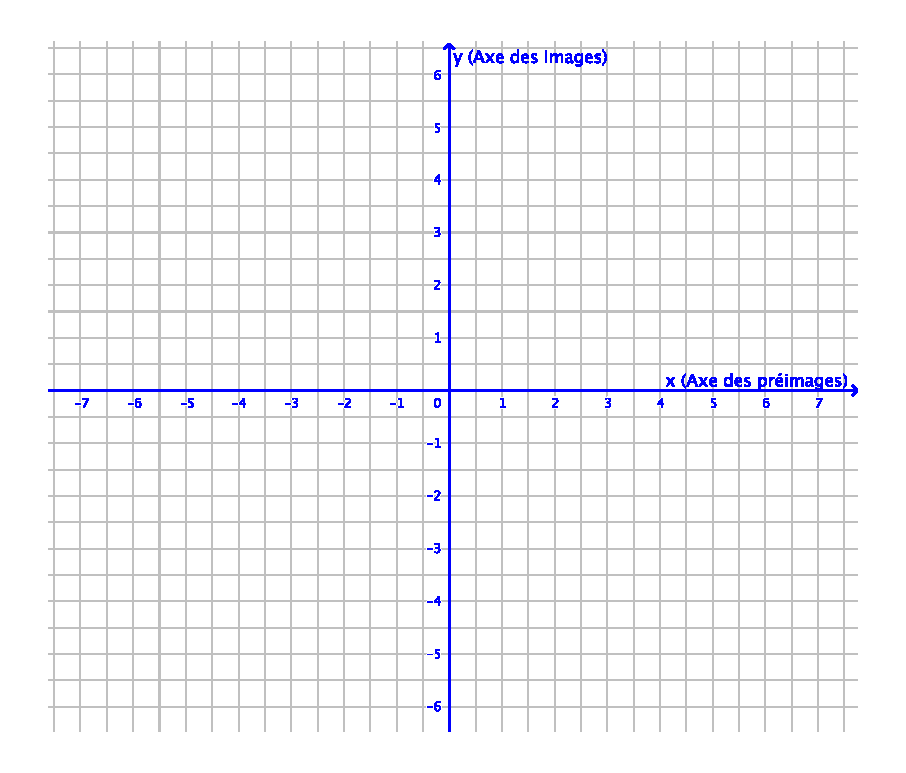
\includegraphics[width=1\textwidth]{media/FA-30/axesvides.pdf}
%\end{center}


\end{enumerate}
}{2}

\exo{
\begin{enumerate}

\item Considérons la fonction $f : x \mapsto -3x$. Recopie dans ton cahier et complète le tableau de valeurs suivants :


\medskip

{\renewcommand{\arraystretch}{1.5}\setlength{\tabcolsep}{.4cm}
\begin{tabular}{|c|c|c|c|c|c|c|c|c|c|c|}\hline
x & -5 & -4 & -3 & -2 & -1 & 0 & 1 & 2 & 3 & 4\\\hline
f(x) & & & & & & & & & & \\\hline
\end{tabular}}
\item Construis un système d'axes dans ton cahier (ou utilise l'un des systèmes d'axes en annexe) et place les points obtenus précédemment. Qu'observes-tu ?

%\begin{center}
%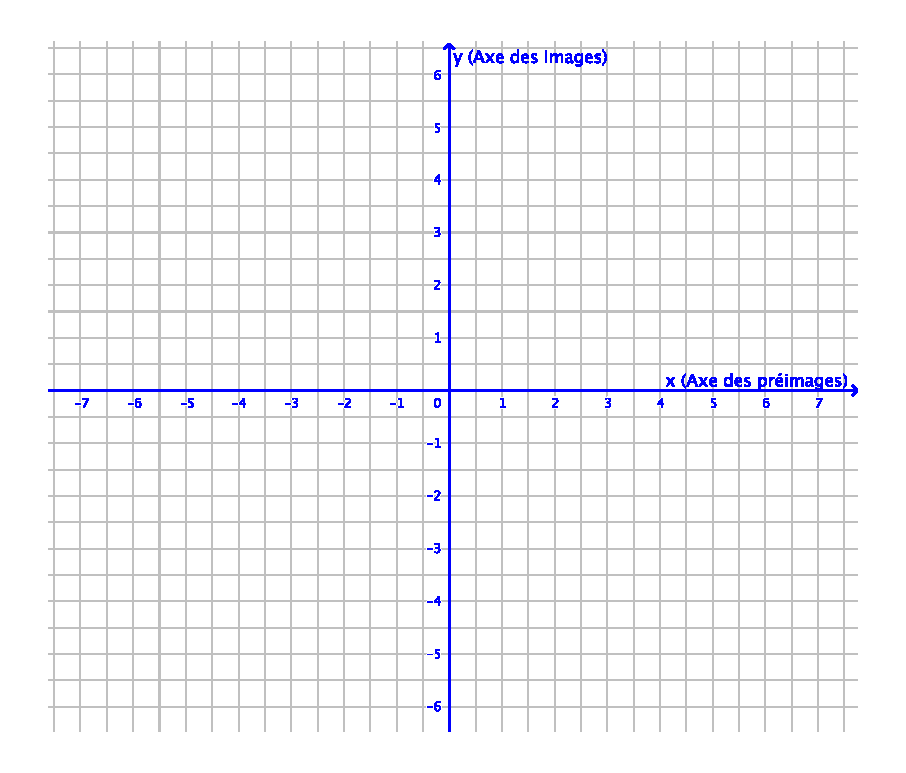
\includegraphics[width=1\textwidth]{media/FA-30/axesvides.pdf}
%\end{center}


\end{enumerate}
}{2}

\exo{
\begin{enumerate}

\item Considérons la fonction $f : x \mapsto -3x+1$. Recopie dans ton cahier et complète le tableau de valeurs suivants :


\medskip

{\renewcommand{\arraystretch}{1.5}\setlength{\tabcolsep}{.4cm}
\begin{tabular}{|c|c|c|c|c|c|c|c|c|c|c|}\hline
x & -5 & -4 & -3 & -2 & -1 & 0 & 1 & 2 & 3 & 4\\\hline
f(x) & & & & & & & & & & \\\hline
\end{tabular}}
\item Construis un système d'axes dans ton cahier (ou utilise l'un des systèmes d'axes en annexe) et place les points obtenus précédemment. Qu'observes-tu ?

%\begin{center}
%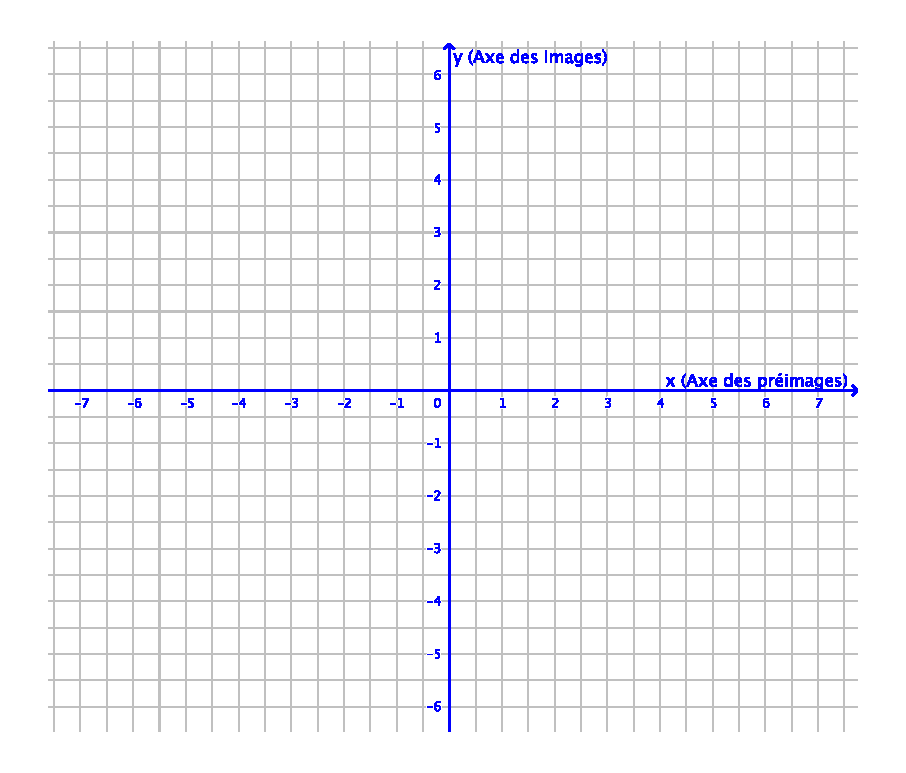
\includegraphics[width=1\textwidth]{media/FA-30/axesvides.pdf}
%\end{center}


\end{enumerate}
}{2}

\exo{
\begin{enumerate}

\item Considérons la fonction $f : x \mapsto 3x+1$. Recopie dans ton cahier et complète le tableau de valeurs suivants :


\medskip

{\renewcommand{\arraystretch}{1.5}\setlength{\tabcolsep}{.4cm}
\begin{tabular}{|c|c|c|c|c|c|c|c|c|c|c|}\hline
x & -5 & -4 & -3 & -2 & -1 & 0 & 1 & 2 & 3 & 4\\\hline
f(x) & & & & & & & & & & \\\hline
\end{tabular}}
\item Construis un système d'axes dans ton cahier (ou utilise l'un des systèmes d'axes en annexe) et place les points obtenus précédemment. Qu'observes-tu ?

%\begin{center}
%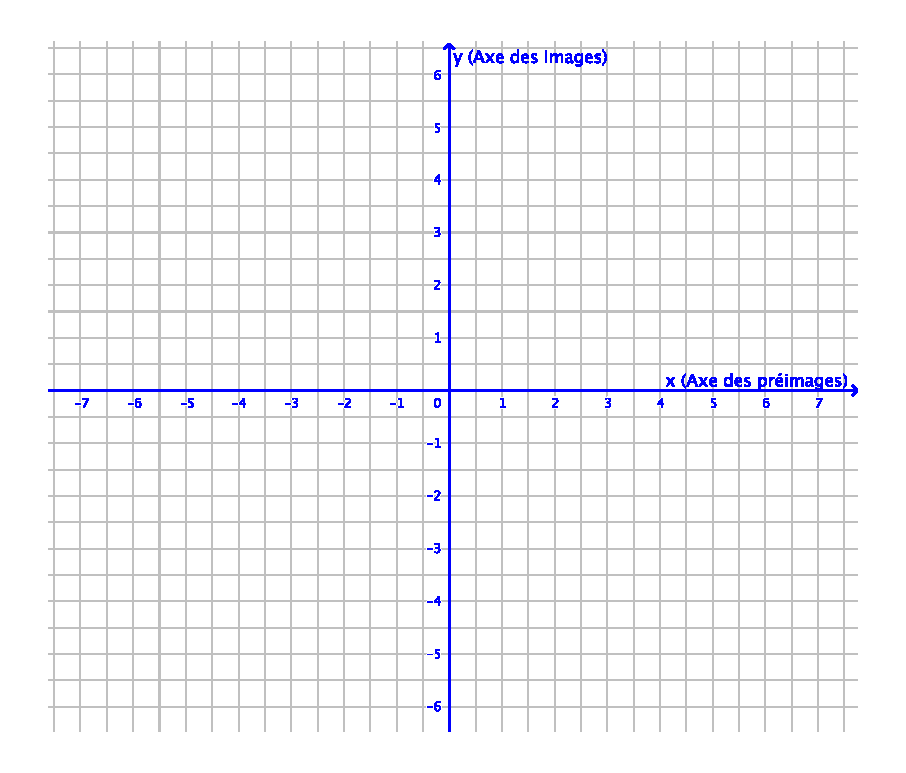
\includegraphics[width=1\textwidth]{media/FA-30/axesvides.pdf}
%\end{center}


\end{enumerate}
}{2}


\exof{FA11}{74}{2}


\newpage

%Fonction affine, linéaire et constante

\resolu{Affine, linéaire ou constante}{Observe les graphiques ci-dessous et complète le tableau en cochant les bonnes réponses :
\begin{center}
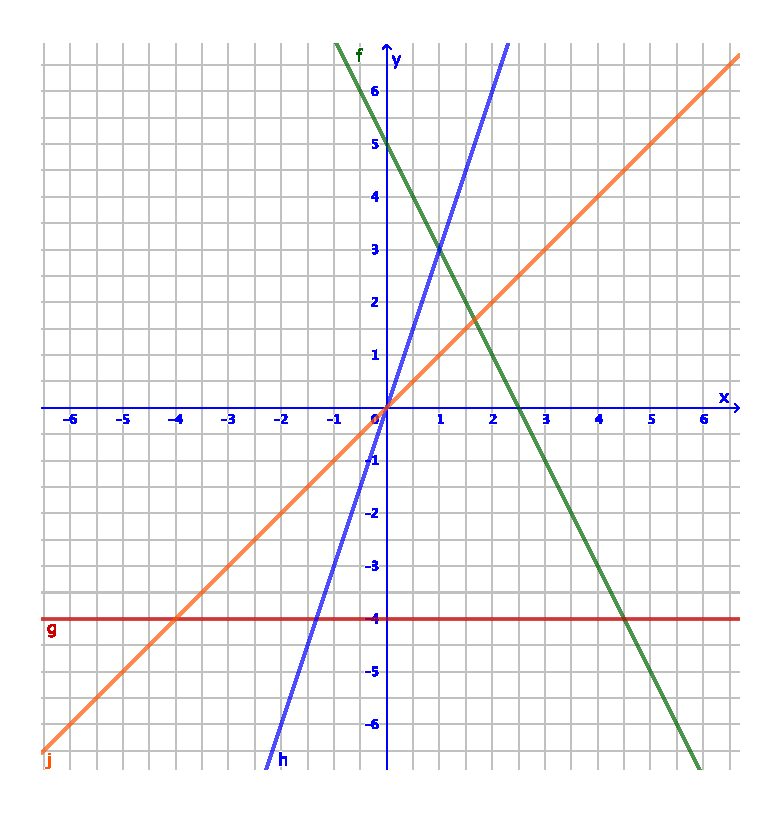
\includegraphics[width=.85\textwidth]{media/FA-30/axesfghj.pdf}
\end{center}

\begin{center}
\begin{tabular}{|l|c|c|c|}\hline
\multicolumn{1}{|c|}{$\nearrow$}& ... affine. & ... linéaire. & ... constante. \\\hline
La fonction $f$ est ... 	&  x	& 		& 		\\\hline
La fonction $g$ est ... 	&  x	& 		& x 	\\\hline
La fonction $h$ est ... 	&  x	& 	x	& 		\\\hline
La fonction $j$ est ... 	&  x	& 	x	& 		\\\hline
\end{tabular}
\end{center}
}{2}

\exop{Observe les graphiques ci-dessous et complète le tableau en cochant les bonnes réponses :
\begin{center}
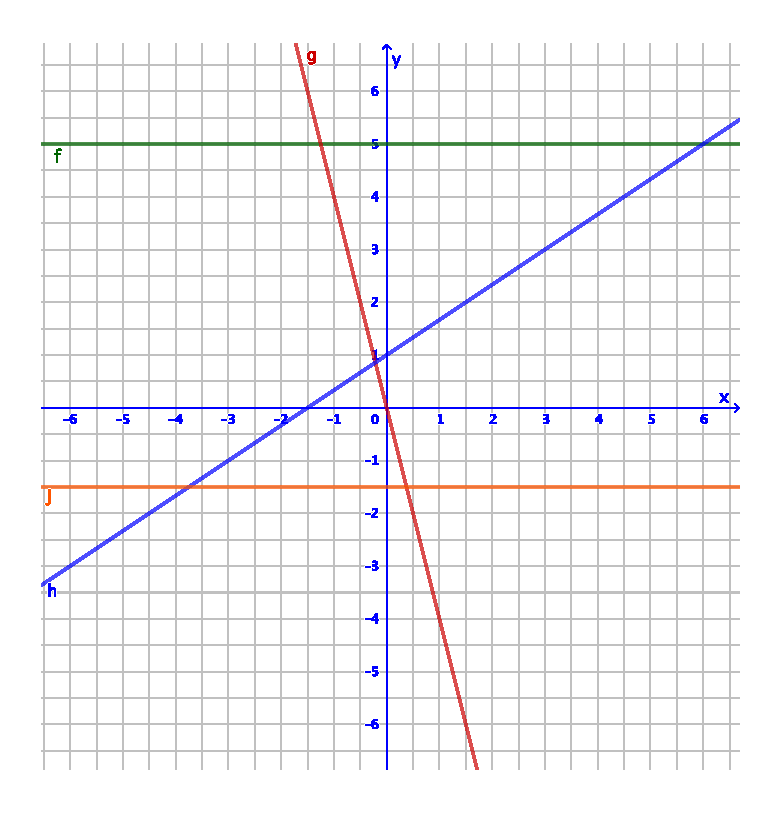
\includegraphics[width=.85\textwidth]{media/FA-30/axesfghj1.pdf}
\end{center}
\begin{center}
\begin{tabular}{|l|c|c|c|}\hline
\multicolumn{1}{|c|}{$\nearrow$}& ... affine. & ... linéaire. & ... constante. \\\hline
La fonction $f$ est ... &  & & \\\hline
La fonction $g$ est ... &  & & \\\hline
La fonction $h$ est ... &  & & \\\hline
La fonction $j$ est ... &  & & \\\hline
\end{tabular}
\end{center}

}{2}

%%%% Ajouter des exercices du voculaires pente et ordonées à l'origine
%%%%%%%%%%%%%%%%%%%%%%%%%%%%%%%


\resolu{Vocabulaire}{On considère les fonctions affines $f, g, h $ dont voici les expressions fonctionnelles.
\begin{center}
$\begin{array}{cp{1cm}cp{1cm}c}
f : x \mapsto 2x-1 & & g : x \mapsto -5x & & h : x \mapsto 3 \\
\end{array}$
\end{center}
Réponds aux questions suivantes.
\begin{enumerate}
\item Quelle est la pente de la fonction $f$ ?

{\bf Réponse :} La pente de la fonction $f$ vaut 2. 
\item Quelle est l'ordonnée à l'origine de la fonction $f$ ?

{\bf Réponse :} L'ordonnée à l'origine de la fonction $f$ vaut -1.
\item Quelle est la pente de la fonction $g$ ? 

{\bf Réponse :} La pente de la fonction $g$ vaut -5.
\item Quelle est l'ordonnée à l'origine de la fonction $g$ ?

{\bf Réponse :} L'ordonnée à l'origine de la fonction $g$ vaut 0, donc cette fonction affine est également une fonction linéaire.
\item Quelle est la pente de la fonction $h$ ? 

{\bf Réponse :} La pente de la fonction $h$ vaut 0, donc cette fonction affine est également une fonction constante.
\item Quelle est l'ordonnée à l'origine de la fonction $h$ ?

{\bf Réponse :} L'ordonnée à l'origine de la fonction $h$ vaut 3.
\end{enumerate}
}{2}

\newpage

\exo{On considère les fonctions affines $f, g, h $ dont voici les expressions fonctionnelles.
\begin{center}
$\begin{array}{cp{1cm}cp{1cm}c}
f : x \mapsto -3x+7 & & g : x \mapsto -3 & & h : x \mapsto -4x \\
\end{array}$
\end{center}
Réponds aux questions suivantes.
\begin{enumerate}
\item Quelle est la pente de la fonction $f$ ? 
\item Quelle est l'ordonnée à l'origine de la fonction $f$ ?
\item Quelle est la pente de la fonction $g$ ? 
\item Quelle est l'ordonnée à l'origine de la fonction $g$ ?
\item Quelle est la pente de la fonction $h$ ? 
\item Quelle est l'ordonnée à l'origine de la fonction $h$ ?
\end{enumerate}
}{2}

\resolu{Expression fonctionnelle}{Donne l'expression fonctionnelle de chaque fonction décrite ci-dessous :
\begin{enumerate}
\item La fonction $a$ est une fonction affine dont la  pente vaut 1 et d'ordonnée à l'origine vaut 2.

{\bf Réponse :} L'expression fonctionnelle est $a : x \mapsto x+2.$
\item La fonction $b$ est une fonction affine dont la pente vaut -2 et l'ordonnée à l'origine vaut -5.

{\bf Réponse :} L'expression fonctionnelle est $b : x \mapsto -2x-5.$
%\item La fonction $c$ est une fonction affine dont la pente vaut 5 et l'ordonnée à l'origine vaut -4.
%\item La fonction $d$ est une fonction affine dont la pente vaut -3 et l'ordonnée à l'origine vaut -5.
\end{enumerate}
 }{2}
 
 \newpage




\exo{Donne l'expression fonctionnelle de chaque fonction décrite ci-dessous :
\begin{enumerate}
\item La fonction $a$ est une fonction affine dont la  pente vaut -1 et d'ordonnée à l'origine vaut 4.
\item La fonction $b$ est une fonction affine dont la pente vaut 4 et l'ordonnée à l'origine vaut -1.
\item La fonction $c$ est une fonction affine dont la pente vaut -2 et l'ordonnée à l'origine vaut +7.
\item La fonction $d$ est une fonction affine dont la pente vaut 7 et l'ordonnée à l'origine vaut -2.
\end{enumerate}
 }{2}
 
\exo{Si possible, donne l'expression fonctionnelle de chaque fonction décrite ci-dessous :
\begin{enumerate}
\item La fonction $a$ est une fonction affine dont la  pente vaut -2 et d'ordonnée à l'origine vaut 5.
\item La fonction $b$ est une fonction linéaire dont la pente est la même que celle de la fonction $a$.
\item La fonction $c$ est une fonction constante dont la pente est la même que celle de la fonction $a$.
\item La fonction $d$ est une fonction constante dont l'ordonnée à l'origine est la même que celle de la fonction $a$ .
\end{enumerate}
 }{2}
 
 \resolu{L'ordonnée à l'origine}{On a tracé quatre droites parallèles. Associe chaque droite a sa bonne expression fonctionnelle en complétant par $d_1, d_2, d_3$ ou $d_4.$
\begin{center}
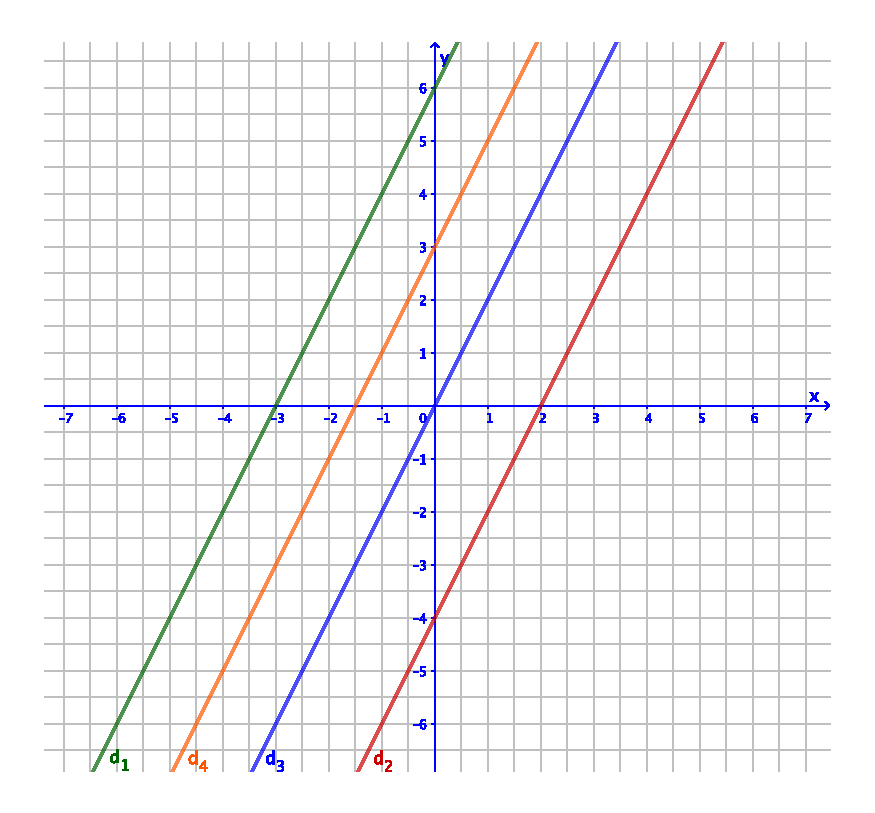
\includegraphics[width=1\textwidth]{media/FA-30/axesd.pdf}
\end{center}
$${\bf d_2} : x \mapsto 2x-4 \qquad\qquad {\bf d_3} : x \mapsto 2x $$
$${\bf d_4} : x \mapsto 2x+3 \qquad\qquad {\bf d_1} : x \mapsto 2x+6 $$
 }{2}
 
 
 \exop{On a tracé quatre droites parallèles. Associe chaque droite a sa bonne expression fonctionnelle en complétant par $d_1, d_2, d_3$ ou $d_4.$
\begin{center}
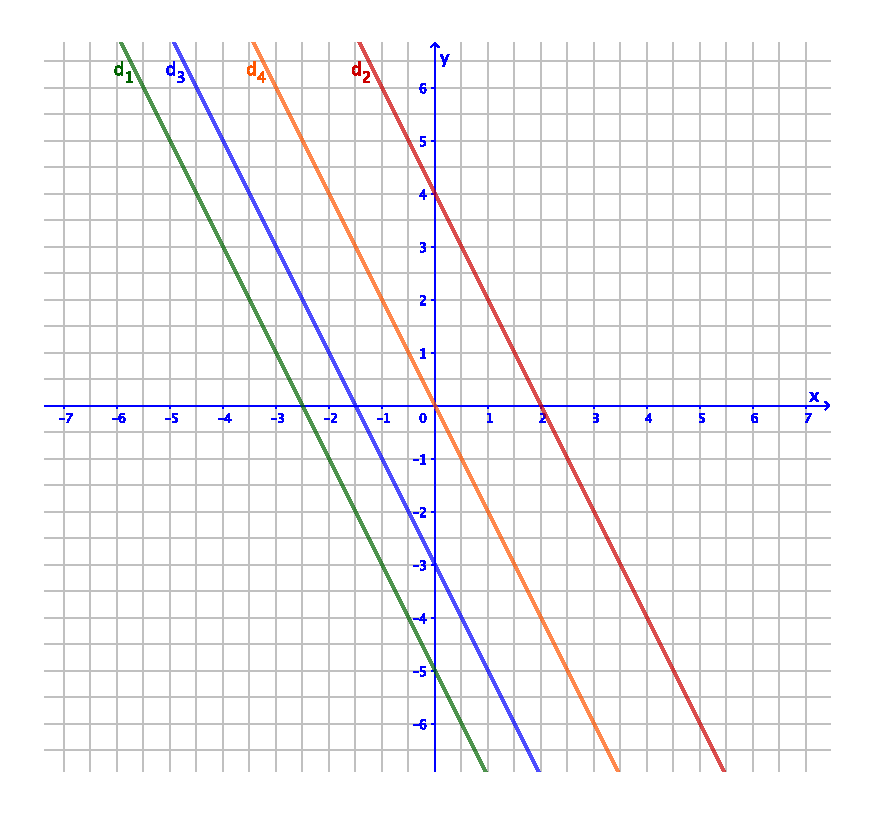
\includegraphics[width=1\textwidth]{media/FA-30/axesd2.pdf}
\end{center}
$$\ligne{1} : x \mapsto -2x-5 \qquad\qquad \ligne{1} : x \mapsto -2x $$

$$\ligne{1} : x \mapsto -2x-3 \qquad\qquad \ligne{1} : x \mapsto -2x+4 $$
 }{2}
 
 
\resolu{La pente}{On a tracé quatre droites concourantes. Associe chaque droite a sa bonne expression fonctionnelle en complétant par $d_1, d_2, d_3$ ou $d_4.$

\begin{center}
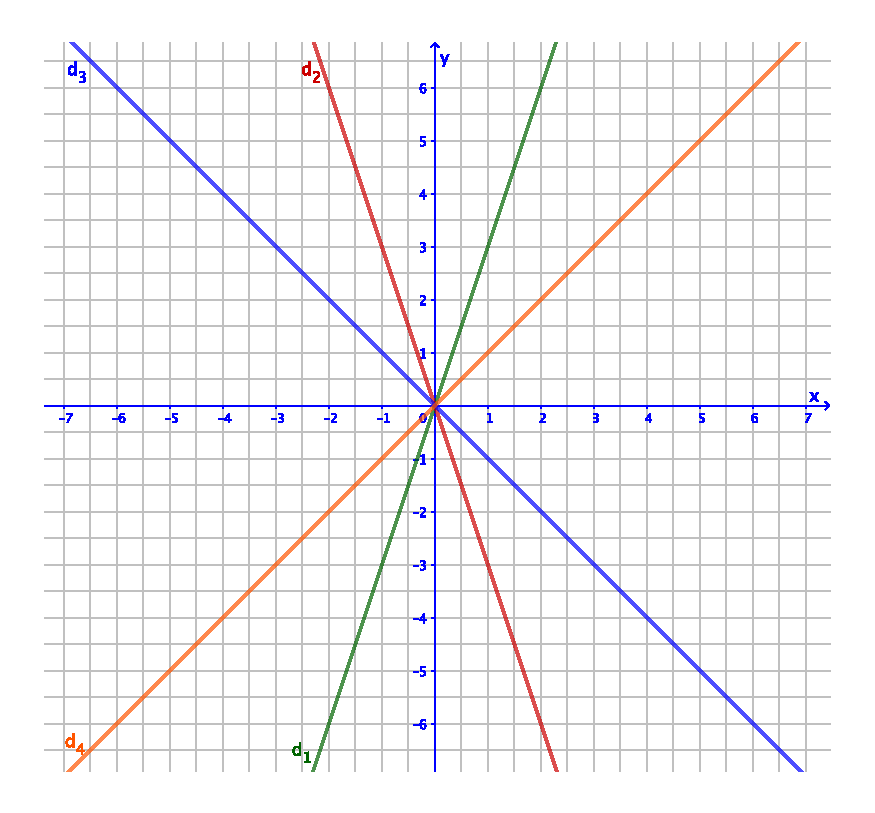
\includegraphics[width=1\textwidth]{media/FA-30/axesd1.pdf}
\end{center}
$${\bf d_2} : x \mapsto -3x \qquad\qquad {\bf d_3} : x \mapsto -x $$
$${\bf d_4} : x \mapsto x \qquad\qquad {\bf d_1} : x \mapsto 3x $$

}{2} 
 
\exop{On a tracé quatre droites concourantes. Associe chaque droite a sa bonne expression fonctionnelle en complétant par $d_1, d_2, d_3$ ou $d_4.$

\begin{center}
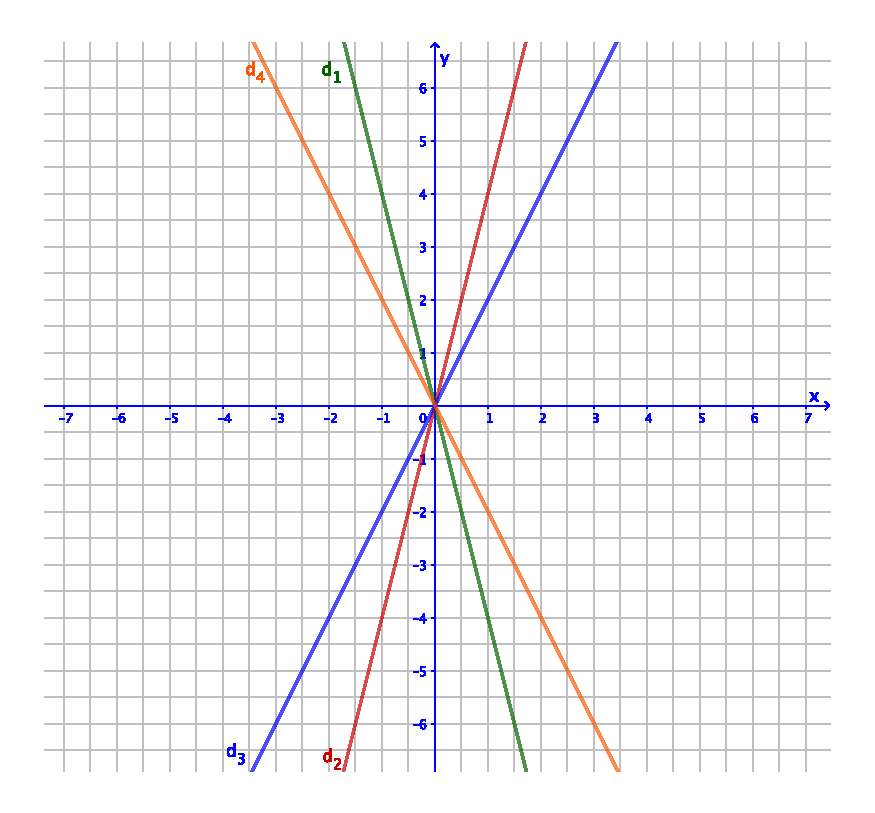
\includegraphics[width=1\textwidth]{media/FA-30/axesd3.pdf}
\end{center}
$$\ligne{1} : x \mapsto -4x \qquad\qquad \ligne{1} : x \mapsto -2x $$

$$\ligne{1} : x \mapsto 2x \qquad\qquad \ligne{1} : x \mapsto 4x $$

}{2}  


\resolu{Vers l'expression fonctionnelle 1}{
Donne l'expression fonctionnelle de la fonction $f$ représentée graphiquement ci-dessous.
\begin{center}
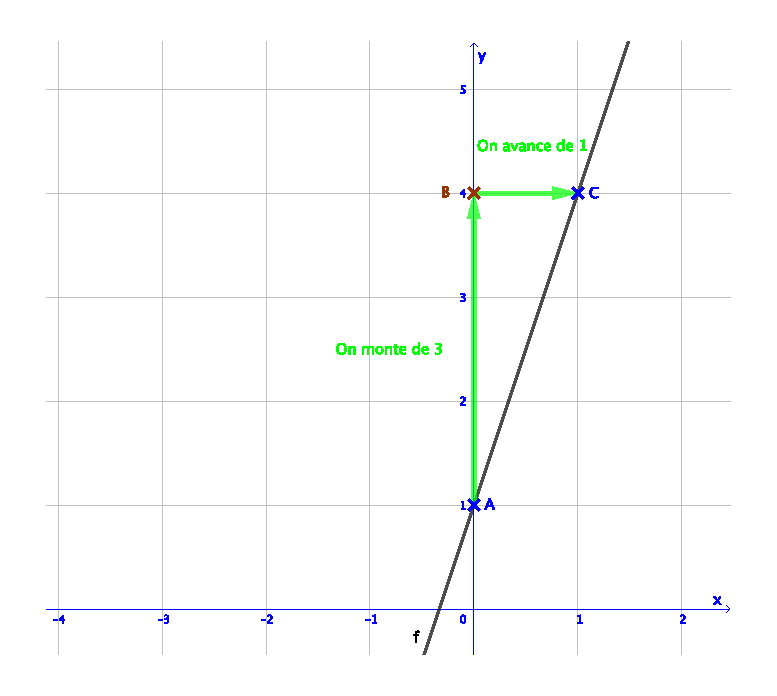
\includegraphics[width=1\textwidth]{media/FA-30/axeszoom2.pdf}
\end{center}
La représentation graphique de cette fonction est une droite, donc il s'agit d'une fonction affine. Par conséquent, on doit déterminer l'ordonnée à l'origine et la pente de cette fonction affine.

On sait que l'ordonnée à l'origine est l'image de zéro, en d'autres termes, il s'agit de la valeur qu'on lit sur l'axe vertical lors de  l'intersection entre l'axe vertical et la droite (la fonction $f$). Ainsi, dans cet exemple, l'ordonnée à l'origine vaut 1.

Pour trouver la pente de cette droite, on part de l'ordonnée à l'origine (point A) et on cherche un deuxième point dont on arrive facilement à lire les coordonnées. Ici, on choisit par exemple le point C. On détermine le déplacement vertical (entre A et B) et le déplacement horizontal (entre B et C).

On doit également se rappeler les règles suivantes :
\begin{itemize}
\item[$\bullet$] Quand on monte verticalement ou on avance horizontalement  le nombre sera positif.
\item[$\bullet$] Quand on descend verticalement ou on recule horizontalement le nombre sera négatif.
\end{itemize}

Ces règles peuvent être symbolisées par le schéma suivant : 

\begin{center}
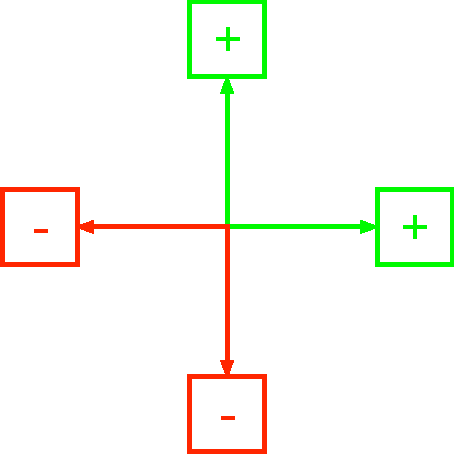
\includegraphics[scale=.75]{media/FA-30/fleches.pdf}
\end{center}

Ainsi, en appliquant la formule de la pente, on obtient :

$$\mbox{pente} = \dfrac{\mbox{distance verticale}}{\mbox{distance horizontale}} = \dfrac{\mbox{\color{green}On monte de 3}}{\mbox{\color{green}On avance de 1}} = \dfrac{\color{green}3}{\color{green}1}=3. $$

Du coup, on vient de trouver que la pente de la fonction $f$ vaut 3 et l'ordonnée à l'origine de la fonction $f$ vaut 1.

Donc : $f : x \mapsto 3x+1.$
}{2}

\resolu{Vers l'expression fonctionnelle 2}{
Donne l'expression fonctionnelle de la fonction $f$ représentée graphiquement ci-dessous.
\begin{center}
\includegraphics[width=1\textwidth]{media/FA-30/axeszoom.pdf}
\end{center}
La représentation graphique de cette fonction est une droite, donc il s'agit d'une fonction affine. Par conséquent, on doit déterminer l'ordonnée à l'origine et la pente de cette fonction affine.

On sait que l'ordonnée à l'origine est l'image de zéro, en d'autres termes, il s'agit de la valeur qu'on lit sur l'axe vertical lors de  l'intersection entre l'axe vertical et la droite (la fonction $f$). Ainsi, dans cet exemple, l'ordonnée à l'origine vaut 4.

Pour trouver la pente de cette droite, on part de l'ordonnée à l'origine (point A) et on cherche un deuxième point dont on arrive facilement à lire les coordonnées. Ici, on choisit par exemple le point C. On détermine le déplacement vertical (entre A et B) et le déplacement horizontal (entre B et C).

On doit également se rappeler les règles suivantes :
\begin{itemize}
\item[$\bullet$] Quand on monte verticalement ou on avance horizontalement  le nombre sera positif.
\item[$\bullet$] Quand on descend verticalement ou on recule horizontalement le nombre sera négatif.
\end{itemize}

Ces règles peuvent être symbolisées par le schéma suivant : 

\begin{center}
\includegraphics[scale=.75]{media/FA-30/fleches.pdf}
\end{center}

Ainsi, en appliquant la formule de la pente, on obtient :

$$\mbox{pente} = \dfrac{\mbox{distance verticale}}{\mbox{distance horizontale}} = \dfrac{\mbox{\color{red}On descend de 2}}{\mbox{\color{green}On avance de 1}} = \dfrac{\color{red}-2}{\color{green}1}=-2. $$

Du coup, on vient de trouver que la pente de la fonction $f$ vaut -2 et l'ordonnée à l'origine de la fonction $f$ vaut 4.

Donc : $f : x \mapsto -2x+4.$
}{2}

\exop{Donne l'expression fonctionnelle de la fonction $f$ représentée graphiquement ci-dessous.

\begin{center}
\includegraphics[width=1\textwidth]{media/FA-30/axeszoom3.pdf}
\end{center}

L'expression fonctionnelle de la fonction $f$ est : 
$$f : x \mapsto \ligne{3} $$

}{2}

\newpage

\exop{Donne l'expression fonctionnelle de la fonction $f$ représentée graphiquement ci-dessous.

\begin{center}
\includegraphics[width=1\textwidth]{media/FA-30/axeszoom4.pdf}
\end{center}

L'expression fonctionnelle de la fonction $f$ est : 
$$f : x \mapsto \ligne{3} $$

}{2}

\newpage

\exop{Donne l'expression fonctionnelle des fonctions $f, g, h$ et $i$ représentées graphiquement ci-dessous.

\begin{center}
\includegraphics[width=1\textwidth]{media/FA-30/axeszoom5.pdf}
\end{center}

L'expression fonctionnelle des fonctions est : 
$$f : x \mapsto \ligne{3} \qquad g : x \mapsto \ligne{3} $$

$$h : x \mapsto \ligne{3} \qquad i : x \mapsto \ligne{3} $$


}{2}

\newpage



\exop{Donne l'expression fonctionnelle des fonctions $f, g, h$ et $i$ représentées graphiquement ci-dessous.

\begin{center}
\includegraphics[width=1\textwidth]{media/FA-30/axeszoom6.pdf}
\end{center}

L'expression fonctionnelle des fonctions est : 
$$f : x \mapsto \ligne{3} \qquad g : x \mapsto \ligne{3} $$

$$h : x \mapsto \ligne{3} \qquad i : x \mapsto \ligne{3} $$

}{2}

\newpage

\resolu{De l'expression fonctionnelle vers le graphique}{Trace sur le système d'axe ci-dessous la fonction $f : x \mapsto -2x+3.$

\begin{center}
\includegraphics[width=1\textwidth]{media/FA-30/axesescalier1.pdf}
\end{center}

Pour tracer une fonction affine, on commence par placer l'ordonnée à l'origine qui correspond à l'image de zéro sur le système d'axe. Donc notre cas, l'ordonnée à l'origine vaut +3, donc on sait que le point A(0,3) est un point appartenant à  la représentation graphique de cette fonction affine $f$ qui est une droite.

Comme une droite est obligatoirement définie s'il on connaît deux points distincts, il suffit de trouver un deuxième point lui appartenant. Pour l'obtenir, on doit utiliser la définition de la pente  et sa valeur pour notre fonction $f$, c'est-à-dire dans notre cas -2.
En nous aidant de nos règles déjà vu précédemment, 
\begin{center}
\includegraphics[scale=.75]{media/FA-30/fleches.pdf}
\end{center}

et en appliquant la définition de la pente en partant de notre point A (l'ordonnée à l'origine),

$$\mbox{pente} = \dfrac{\mbox{distance verticale}}{\mbox{distance horizontale}} = -2 =  \dfrac{\color{red}-2}{\color{green}1}=\dfrac{\mbox{\color{red}On descend de 2}}{\mbox{\color{green}On avance de 1}} . $$

on obtient de point B. Ensuite on peut tracer la représentation graphique de la fonction $f.$

Si nécessaire, on peut reproduire le même raisonnement à partir du point B, pour obtenir d'autres points, par exemple C en nous déplaçant dans l'autre sens en appliquant un raisonnement analogue :


$$\mbox{pente} = \dfrac{\mbox{distance verticale}}{\mbox{distance horizontale}} = -2 =  \dfrac{\color{green}2}{\color{red}-1}=\dfrac{\mbox{\color{green}On monte de 2}}{\mbox{\color{red}On recule de 1}} . $$
 }{2}

\exo{

 Trace les fonctions suivantes sur un système d'axes dans ton cahier.

$$f : x \mapsto x-2 \qquad\qquad g : x \mapsto -x+2 $$

$$h : x \mapsto x-5 \qquad\qquad i : x \mapsto -x+4 $$

\bigskip

%\begin{center}
%\includegraphics[width=1\textwidth]{media/FA-30/axesvides1.pdf}
%\end{center}

}{2}



\exo{

Trace les fonctions suivantes sur un système d'axes dans ton cahier.

$$f : x \mapsto 2x \qquad\qquad g : x \mapsto 2x-3 $$

$$h : x \mapsto -2x \qquad\qquad i : x \mapsto -2x+4 $$

\bigskip

%\begin{center}
%\includegraphics[width=1\textwidth]{media/FA-30/axesvides1.pdf}
%\end{center}
}{2}




\exo{

Trace les fonctions suivantes sur un système d'axes dans ton cahier.

$$f : x \mapsto x+4 \qquad\qquad g : x \mapsto -3x $$

$$h : x \mapsto +5 \qquad\qquad i : x \mapsto -x-1 $$

\bigskip

%\begin{center}
%\includegraphics[width=1\textwidth]{media/FA-30/axesvides1.pdf}
%\end{center}
}{2}



\exo{

 Trace les fonctions suivantes sur un système d'axes dans ton cahier.

$$f : x \mapsto -x+1 \qquad\qquad g : x \mapsto 3x $$

$$h : x \mapsto -5 \qquad\qquad i : x \mapsto x-1 $$

\bigskip

%\begin{center}
%\includegraphics[width=1\textwidth]{media/FA-30/axesvides1.pdf}
%\end{center}
}{2}



\exo{
Trace les fonctions suivantes sur un système d'axes dans ton cahier.

$$f : x \mapsto \frac23x \qquad\qquad g : x \mapsto \frac32x $$

$$h : x \mapsto -\frac32x \qquad\qquad i : x \mapsto -\frac23x $$

\bigskip

%\begin{center}
%\includegraphics[width=1\textwidth]{media/FA-30/axesvides1.pdf}
%\end{center}
}{3}



\exo{

Trace les fonctions suivantes sur un système d'axes dans ton cahier.

$$f : x \mapsto \frac35x \qquad\qquad g : x \mapsto \frac35x-4 $$

$$h : x \mapsto -\frac53x \qquad\qquad i : x \mapsto -\frac53x+2 $$

\bigskip

%\begin{center}
%\includegraphics[width=1\textwidth]{media/FA-30/axesvides1.pdf}
%\end{center}
}{3}



\newpage

\resolu{Résoudre graphiquement}{Résous graphiquement l'équation $3x+2=-x-6$ à l'aide du système d'axes ci-dessous.

\begin{center}
\includegraphics[width=1\textwidth]{media/FA-30/axesinter1.pdf}
\end{center}

Pour résoudre graphiquement une équation, il faut définir le membre de gauche de l'équation comme la fonction $f$ et le membre de droite comme la fonction $g,$ puis tracer les deux fonctions sur le système d'axes. Ainsi, pour notre énoncé, on définit et on trace les fonctions $f(x)=3x+2$ et $g(x)=-x-6.$

La coordonnée $x$ du point d'intersection $I$ correspond à la solution de l'équation. Ainsi, dans notre cas, les coordonnées du point d'intersection $I$ sont  (-2;-4). Donc la solution de l'équation $3x+2=-x-6$ est -2, qu'on peut noter $\mathcal{S}=\lbrace-2\rbrace$ .

}{2}

\exop{Résous graphiquement l'équation $x+3=-2x+6$ à l'aide d'un système d'axes.

%\begin{center}
%\includegraphics[width=1\textwidth]{media/FA-30/axesvides.pdf}
%\end{center}

}{2}

\exop{Résous graphiquement l'équation $x-6=-3x+6$ à l'aide d'un système d'axes.

%\begin{center}
%\includegraphics[width=1\textwidth]{media/FA-30/axesvides.pdf}
%\end{center}

}{2}


\exop{Résous graphiquement l'équation $-2x-6=4x+6$ à l'aide d'un système d'axes.

%\begin{center}
%\includegraphics[width=1\textwidth]{media/FA-30/axesvides.pdf}
%\end{center}

}{2}

\newpage


\exop{
\begin{enumerate}

\item Considérons la fonction $f : x \mapsto x^2$. Complète le tableau de valeurs suivants :


\medskip

{\renewcommand{\arraystretch}{1.5}\setlength{\tabcolsep}{.4cm}
\begin{tabular}{|c|c|c|c|c|c|c|c|c|c|c|c|}\hline
x & -5 & -4 & -3 & -2 & -1 & 0 & 1 & 2 & 3 & 4& 5\\\hline
f(x) & & & & & & & & & & & \\\hline
\end{tabular}}
\item Place les points sur le système d'axes ci-dessus et trace la courbe de cette fonction.
\end{enumerate}

\begin{center}
\includegraphics[width=1\textwidth]{media/FA-30/axesvides2.pdf}
\end{center}
}{2}

\newpage

\exop{
\begin{enumerate}

\item Considérons la fonction $f : x \mapsto -x^2$. Complète le tableau de valeurs suivants :


\medskip

{\renewcommand{\arraystretch}{1.5}\setlength{\tabcolsep}{.4cm}
\begin{tabular}{|c|c|c|c|c|c|c|c|c|c|c|c|}\hline
x & -5 & -4 & -3 & -2 & -1 & 0 & 1 & 2 & 3 & 4& 5\\\hline
f(x) & & & & & & & & & & & \\\hline
\end{tabular}}
\item Place les points sur le système d'axes ci-dessus et trace la courbe de cette fonction.
\end{enumerate}

\begin{center}
\includegraphics[width=1\textwidth]{media/FA-30/axesvides3.pdf}
\end{center}
}{2}





\newpage


\exop{
\begin{enumerate}

\item Considérons la fonction $f : x \mapsto 2x^2$. Complète le tableau de valeurs suivants :


\medskip

{\renewcommand{\arraystretch}{1.5}\setlength{\tabcolsep}{.4cm}
\begin{tabular}{|c|c|c|c|c|c|c|c|c|c|c|c|}\hline
x & -5 & -4 & -3 & -2 & -1 & 0 & 1 & 2 & 3 & 4& 5\\\hline
f(x) & & & & & & & & & & & \\\hline
\end{tabular}}
\item Place les points sur le système d'axes ci-dessus et trace la courbe de cette fonction.
\end{enumerate}

\begin{center}
\includegraphics[width=1\textwidth]{media/FA-30/axesvides4.pdf}
\end{center}
}{2}

\newpage

\exop{
\begin{enumerate}

\item Considérons la fonction $f : x \mapsto -2x^2$. Complète le tableau de valeurs suivants :


\medskip

{\renewcommand{\arraystretch}{1.5}\setlength{\tabcolsep}{.4cm}
\begin{tabular}{|c|c|c|c|c|c|c|c|c|c|c|c|}\hline
x & -5 & -4 & -3 & -2 & -1 & 0 & 1 & 2 & 3 & 4& 5\\\hline
f(x) & & & & & & & & & & & \\\hline
\end{tabular}}
\item Place les points sur le système d'axes ci-dessus et trace la courbe de cette fonction.
\end{enumerate}

\begin{center}
\includegraphics[width=1\textwidth]{media/FA-30/axesvides5.pdf}
\end{center}
}{2}

\newpage


\vspace*{2cm}


\begin{center}
\includegraphics[width=1\textwidth]{media/FA-30/axesvides1.pdf}
\end{center}



\end{document}
